\chapter{Analysis}
\label{chap:analysis}

By modeling spatially and spectrally resolved obserations of protoplanetary disks, we can measure their chemical and physical characteristics. To model the system, we generate a synthetic image of what a disk with known characteristics (like disk radius, mass, chemical abundances, and so on) would look like at a certain distance, inclination, and position angle relative to us. We can then turn that synthetic image into a synthetic visibility set, and then compare those visibilities to our observations. By iterating this process and varying the value of those input parameters, we are able to generate many models with different parameter combinations, evaluate how well each resulting model disk matches our observations, and find which values best describe our disks.

% It’s not just the aggregation, but rather the iterative process itself that allows us to explore parameter space.  Also, MCMC doesn’t just tell us the best fit values, but, critically, how well we know those values (the uncertainties that we get from the PDF).

In \S\ref{section:gas_model}, we describe the basic equations and computational processes that generate the model disks. In \S\ref{section:param_space}, we describe how, once models are made, we move through high-dimensional parameter space to identify regions of best-fit. Finally, in \S\ref{section:fitting_procedure}, we present the results of our fitting procedures.


\section{Gas Model}
\label{section:gas_model}

In this work, we use a gas-disk model originally developed by \citet{Rosenfeld2012,Rosenfeld2013} and translated from IDL to Python by \cite{Flaherty2015}. The code assumes that Local Thermal Equilibrium\footnote{This may or may not be a valid assumption in protoplanetary disks, but \cite{Pavlyuchenkov2007} showed that it was appropriate for CO.} (LTE), and hydrostatic equilibrium. The code draws on temperature- and surface-density profiles provided by the user to calculate a vertical density structure, and calculates the model disk's velocity field based on the stellar mass. It then performs radiative transfer on the resulting structure to create a sky-projected image of the model disk, taking into account thermal and turbulent line broadening. The assumption of LTE allows the code is able to to run quickly enough to allow for a Markov Chain Monte Carlo routine to generate models on a reasonable timescale, as described in \S\ref{subsection:mcmc}.




\subsection{Establishing Physical Profiles}
\label{subsection:physical_profs}
A circumstellar disk can be characterized by three major profiles: its radial and vertical temperature structures, its radial and vertical density structures, and its velocity field. Generating a model disk is a matter of defining these three functions.


% However, these are complex functions, and the reality that they attempt approximate is not necessarily a well-behaved, simple one; no disk's density actually falls off exponentially, although in some cases it can be well approximated as such (\cite{Hughes2008}, \cite{Williams2011}). Furthermore, even these approximations often cannot be solved analytically, instead relying on numerical integration to be solved, which is a computationally expensive task. Therefore, we choose to make certain simplifying assumptions which, although they come at a cost to realism, enable significantly increased computation speeds.

% Are you specifically talking about the hydrostatic equilibrium condition here?  If so, say it!  I can’t think of anything else that requires numerical integration to solve in the code… unless you’re talking about some sort of arbitrary functional form, but that would not be motivated by theory, and not really by observations either.  There are a lot of good reasons why we assume these functional forms, not just because they’re fast!

% LTE is the only assumption that really increases the computation speed — so if that’s what this paragraph is about you should say it explicitly.  Right now you’re conflating the functional forms of the density/temperature/velocity profiles with the physical assumptions of LTE and hydrostatic equilibrium, so please try to separate those out.  (There is excellent evidence that these disks are well described by a Keplerian velocity profile in hydrostatic equilibrium — that’s basically what Katherine Rosenfeld’s 2013 paper on HD 163296 was about!).  

% Wait, what?  That’s not what LTE means.  Also, you have a 2-D temperature profile, not a 1-D temperature profile!  Do a little more reading about LTE and try again. :-) REWORK


For the disk's temperature profile, our code uses the parametrization of disk temperature structure first laid out by \citet{Dartois2003}, where the disk's temperature is given by,

\begin{align}
  T_{\text{gas}}(r, z) = \begin{cases}
                          T_a + (T_m - T_a) \left[ \cos \frac{\pi z}{2 z_q} \right]^{2\delta} \text{   if } z > z_q \\
                          T_a \text{   if } z \leq z_q(r).
                         \end{cases}
\end{align}
\label{eqn:temp_str}

$\delta$, a tunable exponent controlling the rate of the disk's vertical temperature decay, is set to 1 as in \citet{Factor2017}, though it can take on values between 1-2 \citep{Dartois2003}. The atmospheric temperature and mid-plane temperatures are given by $T_a$ = $T_\text{atm,150} (r/150 \text{AU})^{q}$ and $T_m$ = $T_\text{mid, 150} (r/150 AU)^{q}$, where $q$ is typically negative and controls the functions' decay. Since $T_m$ is smaller than $T_a$, the second term of the low-scale height temperature function is negative, so the sinusoid effectively implements a decreasingly-negative contribution to the temperature with hight above midplane.  The disk's scale height, controlled by $z_q$, is assumed to be radially increasing, as described by a power law, $z_q(r) = z_{q,150}(r/150 \text{AU})^{1.3}$.


The disk's velocity field is assumed to be Keplerian with slight corrections for gas pressure support and the addition of a vertical dependence. The assumption of Keplerian veloicites is generally valid in the case that $M_{\text{disk}} \ll M_{\star}$, which continuum observations of the system have shown to be the case for these disks. With these corrections added, the model disk's velocity field is given by


\begin{align}
  \frac{v_\phi^2}{r} = \frac{GM_\star r}{(r + z)^{3/2}} + \frac{1}{\rho_\text{gas}} \frac{\partial P_\text{gas}}{\partial r};\,\, v_r = v_z = 0.
\end{align}


The final structure we would like to define is the disk's gas density profile. By assuming hydrostatic equilibrium, we may relate the disk's gas density and temperature profiles as

\begin{align}
  -\frac{\partial \ln \rho_\text{gas}}{\partial z} = \frac{\partial \ln T_\text{gas}}{\partial z} + \frac{1}{c_s^2} \left[\frac{G M_{\*} z}{(r^2 + z^2)^{3/2}} \right].
\end{align}

Here $c_s$ is the local sound speed, given by $c_s^2 = \frac{k_B T_\text{gas}}{\mu m_H}$, $T_\text{gas}$ is the temperature profile given above, $m_H$ the mass of hydrogen, and $\mu$ is the mean molecular weight of the gas, set here at 2.37 to reflect the gas's 80\% H$_2$ composition. We may solve this equation by integration, giving us the disk's density profile $\rho(r, z)$.


The model's surface density profile is drawn from \citet{Hartmann1998}, in which they expanded on the work of \citet{LyndenBell1974} to show that the structure of an isolated disk with viscosity given by $\nu \propto R^\gamma$ is well-described by


% Also, isn't this Hughes2008's equation?

\begin{align}
  \Sigma_{\text{gas}}(r) = \frac{M_{\text{gas}} (2 - \gamma)}{2 \pi R_c^2} \left(\frac{r}{R_c} \right)^{-\gamma} \exp \left[-\left(\frac{r}{R_c} \right)^{2-\gamma} \right],
\end{align}

\noindent
where $R_c$ is the radial extent of the gas disk, $\gamma$ is a power law index, and $M_\text{gas}$ is the total gas mass. This form allows the disk to behave as a power law radially until R$_c$, at which point it turns over into exponential decay. \citet{Hughes2008} showed that exponentially tapering the disk's outer radius, rather than sharply cutting it, provides the best agreement between gas and disk outer radii. We approximate $M_\text{gas} = M_\text{disk}$, since at this early stage in the disk's development, the gas is by far the majority element of the disk's mass total (although, as discussed in \S\ref{chap:introduction}, this assumption has come under scrutiny in recent years).

% REWORK (on temp freezeout dropoff): Hm, this reminds me that Charlie Qi recently showed that freeze-out is less abrupt than this, so we should probably do something a bit more gradual for freeze-out (I thought Kevin had implemented this, but maybe not in the version of the code that you’re using).  It’s not extremely high-priority, but you should check out Charlie’s (Chunhua’s) papers and make sure you know what I”m talking about and then think about how we could do this better.  


Modifications are made to this density profile in two cases. At sufficiently low temperatures, molecules will condense out of the gas phase. The mid-plane of the disk is sufficiently cold to prompt this behavior. We simulate this behavior by dropping the gas density by a factor of $10^{-18}$ wherever the temperature falls below some characteristic freeze-out temperature, T$_{FO}$, a temperature which is molecule-specific. Conversely, at the disk's upper surface, photodissociation by stellar and interstellar radiation dominates, so we implement a decrease in density wherever the hydrogen column density at the disk's surface falls below a characteristic value. We use values drawn from \cite{Factor2017} for these parameters, presented in Table \ref{tab:mol_specifics}.


\begin{table}
  \begin{threeparttable}
    \centering
    \caption{Molecule-specific values}
    \label{tab:mol_specifics}
    \renewcommand{\arraystretch}{1.2}
    \begin{tabular}{c  l  c c }
      \toprule \toprule
      \multirow{2}{*}{Parameter} & \multirow{2}{*}{Description}    & \multicolumn{2}{c}{Fixed Value(s)} \\
                                 &                                 & CO, HCO$^+$ & HCN \\
      \midrule %\midrule
      T$_{FO}$ (K)           &  Molecular freeze-out temperature   &  19 & 60    \\
      $\sigma_\text{Max}$ (cm$^{-2}$) & Column density upper limit &  $1.3 \times 10^{30}$ & $9.5 \times 10^{21}$  \\
      \bottomrule
    \end{tabular}
    \begin{tablenotes}\footnotesize
      \item[*] Values drawn from \cite{Factor2017}
    \end{tablenotes}
  \end{threeparttable}
\end{table}



% \begin{figure}[htp]
% \centering
%   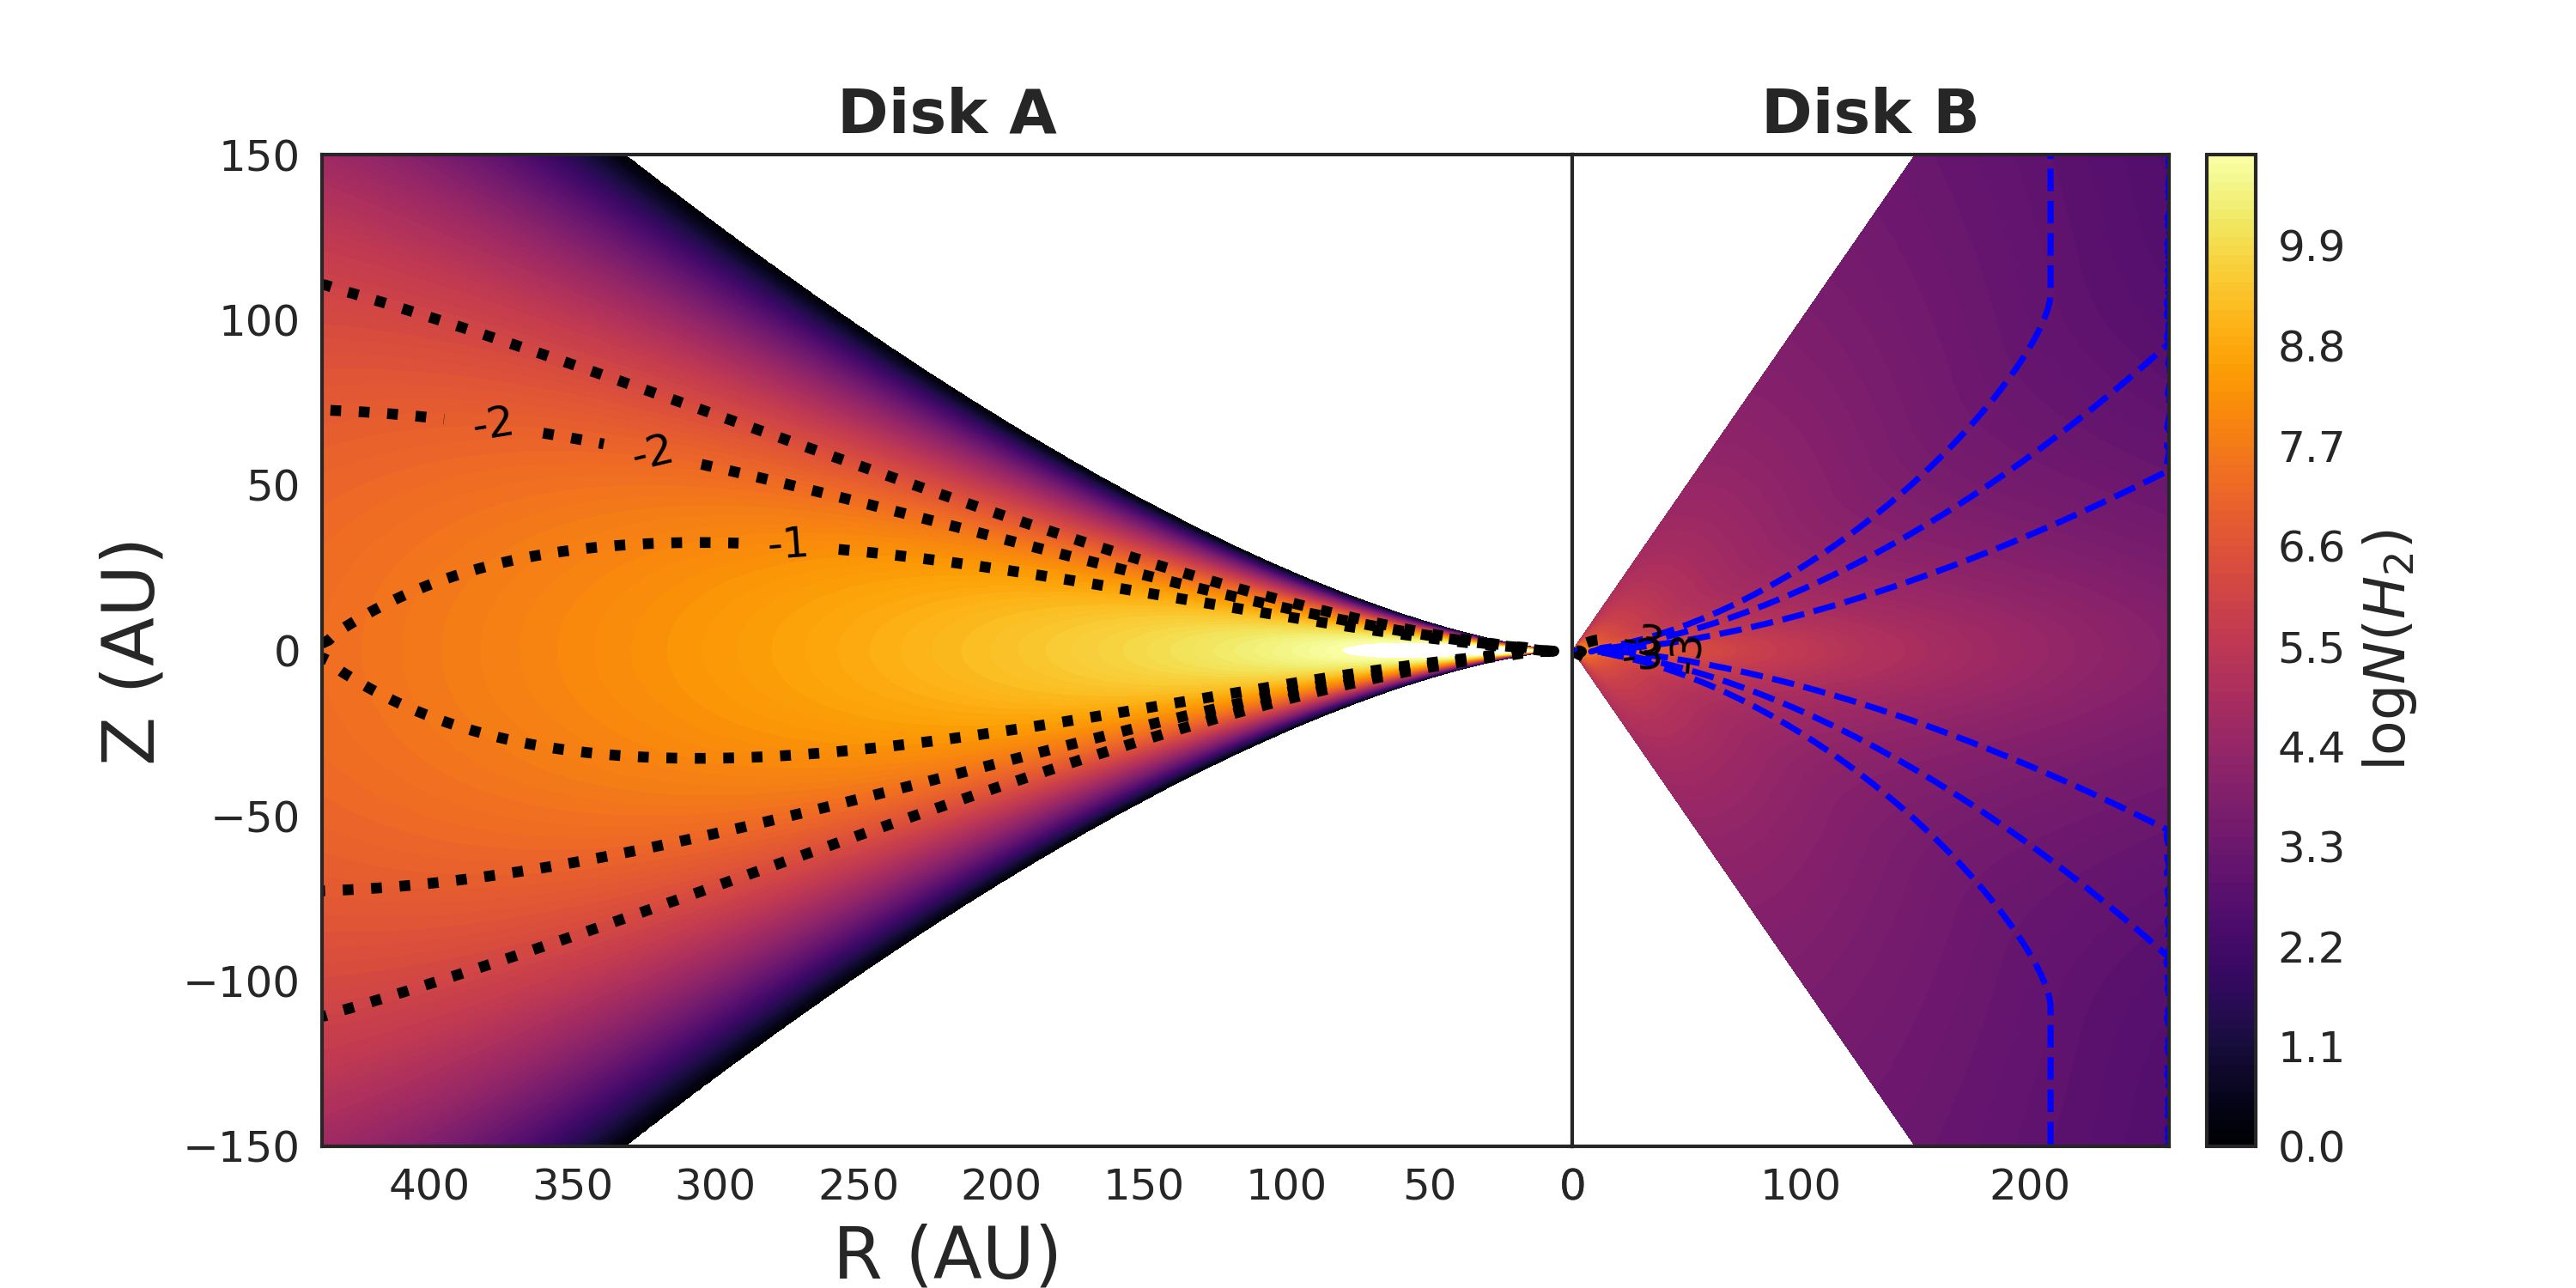
\includegraphics[width=\linewidth]{example-disk-strs.png}
%   \captionof{figure}{Radial and vertical temperature structures for disk A \textit{(left)} and disk B \textit{(right)} in CO. We may quickly see that disk A has a larger radial extent and a better defined profile, thanks to its higher signal.}
%   \label{fig:temp_dens_str}
% \end{figure}
% REWORK: Need a much more informative caption!  Check Sam’s paper for examples if you need them. Also, make the labels bigger on the color bar to the right for readability.  Add units to the label too (both on the color bar and on the contours in the figure).





\subsection{Generating a Model Image}

Having now established our model disk's physical structure through temperature, density, and velocity profiles, flux contributions through the disk are calculated. To do so, we find specific intensity by integrating the equation of radiative transfer:

\begin{align}
  I_\nu = \int_0^{\infty} K_\nu(s)\ S_\nu(s)\ e^{-\tau_\nu(s)}\ ds,
\end{align}

where $K_\nu(s)$ is the absorption coefficient, $\tau_\nu(s)$ is the optical depth and is defined as $\tau_\nu(s) = \int_0^s K_\nu(s') ds'$, and $S_\nu(s)$ is the source function. Since disks emit as blackbodies, the Planck function, $B_\nu(T)$, is used as the source function. Line broadening, a function of temperature and disk turbulence, is added, and the resulting flux is Doppler shifted to account for the disk's user-specified systemic velocity. Finally, the image is scaled, shifted, and rotated to account for the source's distance ($d$), angular offset from the center of the image ($\Delta \alpha$ and $\Delta \delta$), and position angle and inclination (PA and $i$) relative to our viewing direction.
% REWORK: Add an explanation of how I got positional offsets
% REWORK: Baseline cutoff explanation. Does that happen in a different chapter? Maybe should happen here.

Since the model disk is fully defined at every point in both physical and velocity space, we may set the spatial and spectral resolution to ensure that it is sampled well compared to the resolution of the data. We set our spectral resolution to match that of our observation, while we let the spatial resolution be $\sim$ 1/10 the size of the synthesized beam. This resolution is high enough to avoid sampling artifacts when we simulate interferometric observations of the image.

% REWORK: Random thought as I’m reading this: can you please check whether or not Hanning smoothing is implemented in the MIRIAD commands that Kevin’s code uses?  Before uvmodel, there should be a “hanning” command in MIRIAD… let me know.  (If not, we should add it.)

We then use the Miriad task \texttt{uvmodel} to generate visibilities from the model image, sampled in the same $uv$ tracks as our observation. The $\chi^2$ statistic is then used as a goodness-of-fit metric to compare the data and model in the visibility domain. We make this calculation in the visibility domain, rather than the image domain, so that the resulting $\chi^2$ value is not influenced by artifacts generated in the imaging process.


In summary, we can generate a model disk by calculating its physical structures (in radial temperatures, densities, and velocities), then drawing on radiative transfer to calculate the flux contributions from the disk. That flux is sky-projected to match the observed source's orientation, and the resulting image is then transformed from the image domain to the visibility domain and its fit quality evaluated.



\section{Exploring Parameter Space}
\label{section:param_space}

Now that we have the tools available to generate synthetic images that are tuneable across a large number of parameters, we must decide how best to move through that large parameter space to find a best-fit region. To do so, we use two methods.

\subsection{Grid Search}
\label{subsection:grid_search}
The first, and perhaps most intuitive, way to move through this parameter space is using a simple grid search. A grid search involves manually assembling lists of values to try for each parameter and then generating models and calculating the resulting $\chi^2$ value for every possible combination of parameters in those lists. A best-fit value is recovered by simply finding the point in that $n$-dimensional grid that yielded the best $\chi^2$, and then either calling that position in parameter space a best-fit location or then defining a finer grid around that point and repeating the process until an acceptable resolution has been reached. Benefits of grid search include its relatively straightforward nature (and, consequentially, the relative simplicity of implementating it) and its usefullness as a diagnostic tool, since very specific regions of parameter space may be sampled with the manual entry of positions to test. However, its simplicity leaves room for improvement.

We used grid search to locate the disks in $(\alpha, \delta, v)$ space. All other parameters were fixed at best-guessed values, then grids were run with resolutions sufficiently fine to meet the observations' spatial and spectral resolution. Grids for the disks' systemic velocities were centered at values found in \citet{Williams2014}, while $\Delta \alpha$ and $\Delta \delta$ offsets were first approximated using the MIRIAD task \texttt{uvfit} to fit a Gaussian to each disk. The resulting centroids were used to center the grids for refinement.


\subsection{Markov Chain Monte Carlo}
\label{subsection:mcmc}

Markov Chain Monte Carlo (MCMC) algorithms offer us a way to both sample the probability distribution of a high-dimensional parameter space (much like a grid search), but offers an improvement over grid search by yielding the posterior probability distribution of each point, which allows us to characterize the uncertainty associated with each best-fit value with error bars. We use an affine-invariant formulation of the MCMC algorithm described by \citet{Goodman2010} and implemented in the Python package \texttt{emcee} by \citet{ForemanMackey2013}.

MCMC routines sample the probability distribution of a given $n$-dimensional parameter space by deploying an army of ``walkers." Each walker begins at some initial position, evaluates the $\chi^2$ value of that point, and then proposes moving to a new position in parameter space according to a Gaussian probability distribution centered at the current point and decaying with distance (so that nearer points are preferentially, but not necessarily, selected). The $\chi^2$ value of this new position - or ``step" - is then evaluated, and is either accepted (the walker moves to that position) or rejected (the walker remains where it is and repeats the new-step proposal process) with probability $p = \exp \left[ (\chi_\text{current}^2 - \chi_\text{new}^2)/2 \right]$\footnote{In practice, we take the natural log of both sides of this equation, such that the quantity we are really evaluating is lnprob = $\Delta \chi^2/2$.}. This function indicates that if the proposed step yields a better fit (a lower $\chi^2$ value) than the current position, $p > 1$ and the step is accepted. However, if proposed step results in a worse fit, there is still a non-zero chance that the step is accepted, proportional to how much worse it is. This willingness to accept an increased $\chi^2$ value allows the walker to avoid becoming trapped in local minima. The list of steps taken by each walker and their accompanying $\chi^2$ values are compiled into the ``chain" part of Markov Chain Monte Carlo. \citet{Goodman2010} show that a walker's desire to remain in near a certain position is proportional to that position's local probability density, meaning that we may infer uncertainties in our fits from the density of walker steps taken in a region.

We may introduce boundaries to the parameter space explored by our walkers using ``priors." These priors are manually set, and allow us to restrict the walkers' motions from entering regions that we know a priori to be implausible fits. Justifications for these constraints are either physical (e.g. a disk should not have a negative radius) or observed (e.g. both disks' radii are clearly far less than 1000 AU). These priors may be either uniform, with hard cuts at their bounds (and returning lnprob=-$\inf$), or Gaussian, with preferential treatment given to walkers closer to the Gaussian centroid (a known value). For this work, we implement a Gaussian prior on each disk's position angle in order to guide the search towards the values reported in \citet{Williams2014} but still allow it the flexibility to self correct if necessary. This prior takes the form of a contribution to the log likelihood function, such that:

\begin{align}
  \text{lnprob} = -\chi/2  -\ln{\frac{1}{\sqrt{2 \pi \sigma_{PA}^2}}} \exp{^{\frac{\text{PA}^2}{2 \sigma_{PA}^2}}}
\end{align}

\noindent
for each disk's position angle, where $\sigma_{PA}$ is the position angle uncertainty given by \citet{Williams2014}.



We may visualize the results of the walkers' journeys using corner plots. Corner plots allow high-dimensional space to be visualized in two dimensions by taking slices across each pair of axes and showing the density of samples drawn in that slice. In each of these slices, a perfectly certain fit would appear as a very tight, point-like Gaussian - the sample density around the best fit would be extremely high and low everywhere else, as the walkers quickly converged and remained on that best fit point - while conversely, higher uncertainties are shown by a wide spread of samples around the central point. Degeneracies between parameters can be seen as streaks in these corner plots, showing that a change in one parameter produces a change in the other. Corner plots for Disk A and B in an HCO$^+$ fit are shown in Figs \ref{fig:corner_a} and \ref{fig:corner_b}, respectively.


\begin{figure}[htp]
  % Maximum length
  % \subcaptionbox{1a\label{fig1:a}}{\includegraphics[width=1.6in]{example-image-a}}\hfill%
  % \subcaptionbox{1b\label{fig1:b}}{\includegraphics[width=1.6in]{example-image-a}}%
  % \bigskip
  % Equal length
  \hspace*{\fill}%
  \subcaptionbox{Disk A fits \label{fig:corner_a}}{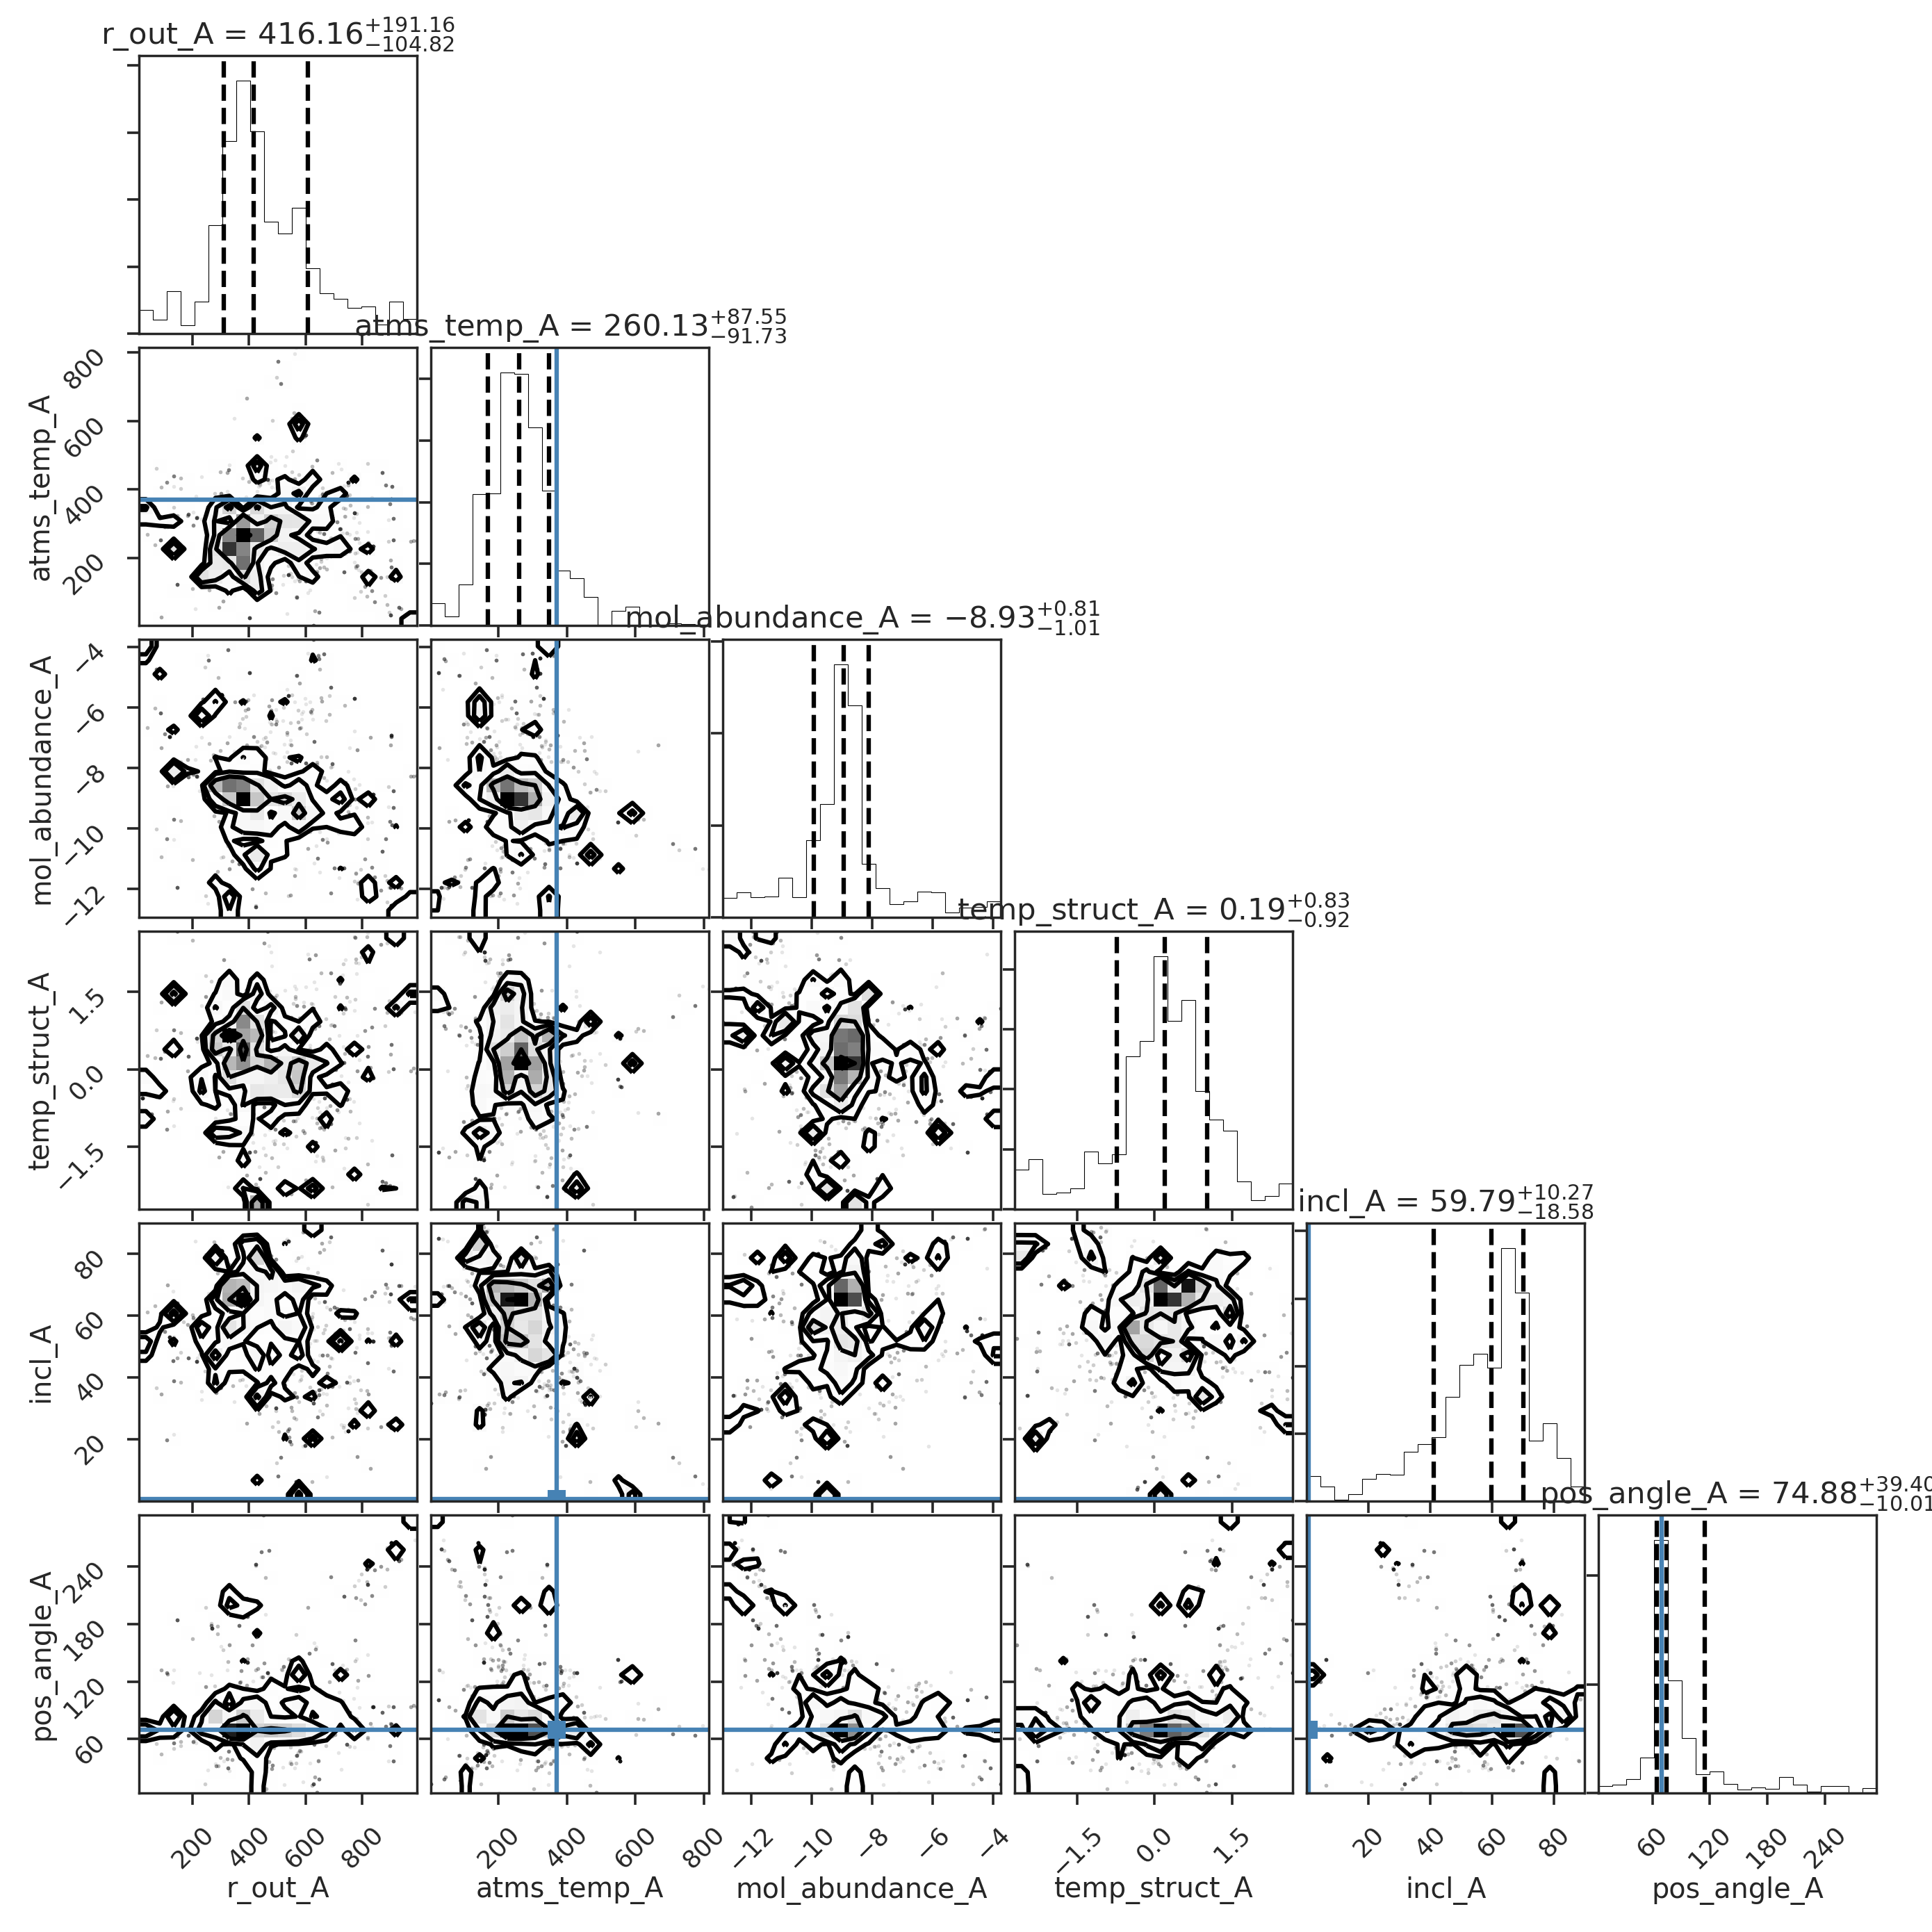
\includegraphics[width=0.49\linewidth]{cornerplot-diskA.png}}\hfill%
  \subcaptionbox{Disk B fits \label{fig:corner_b}}{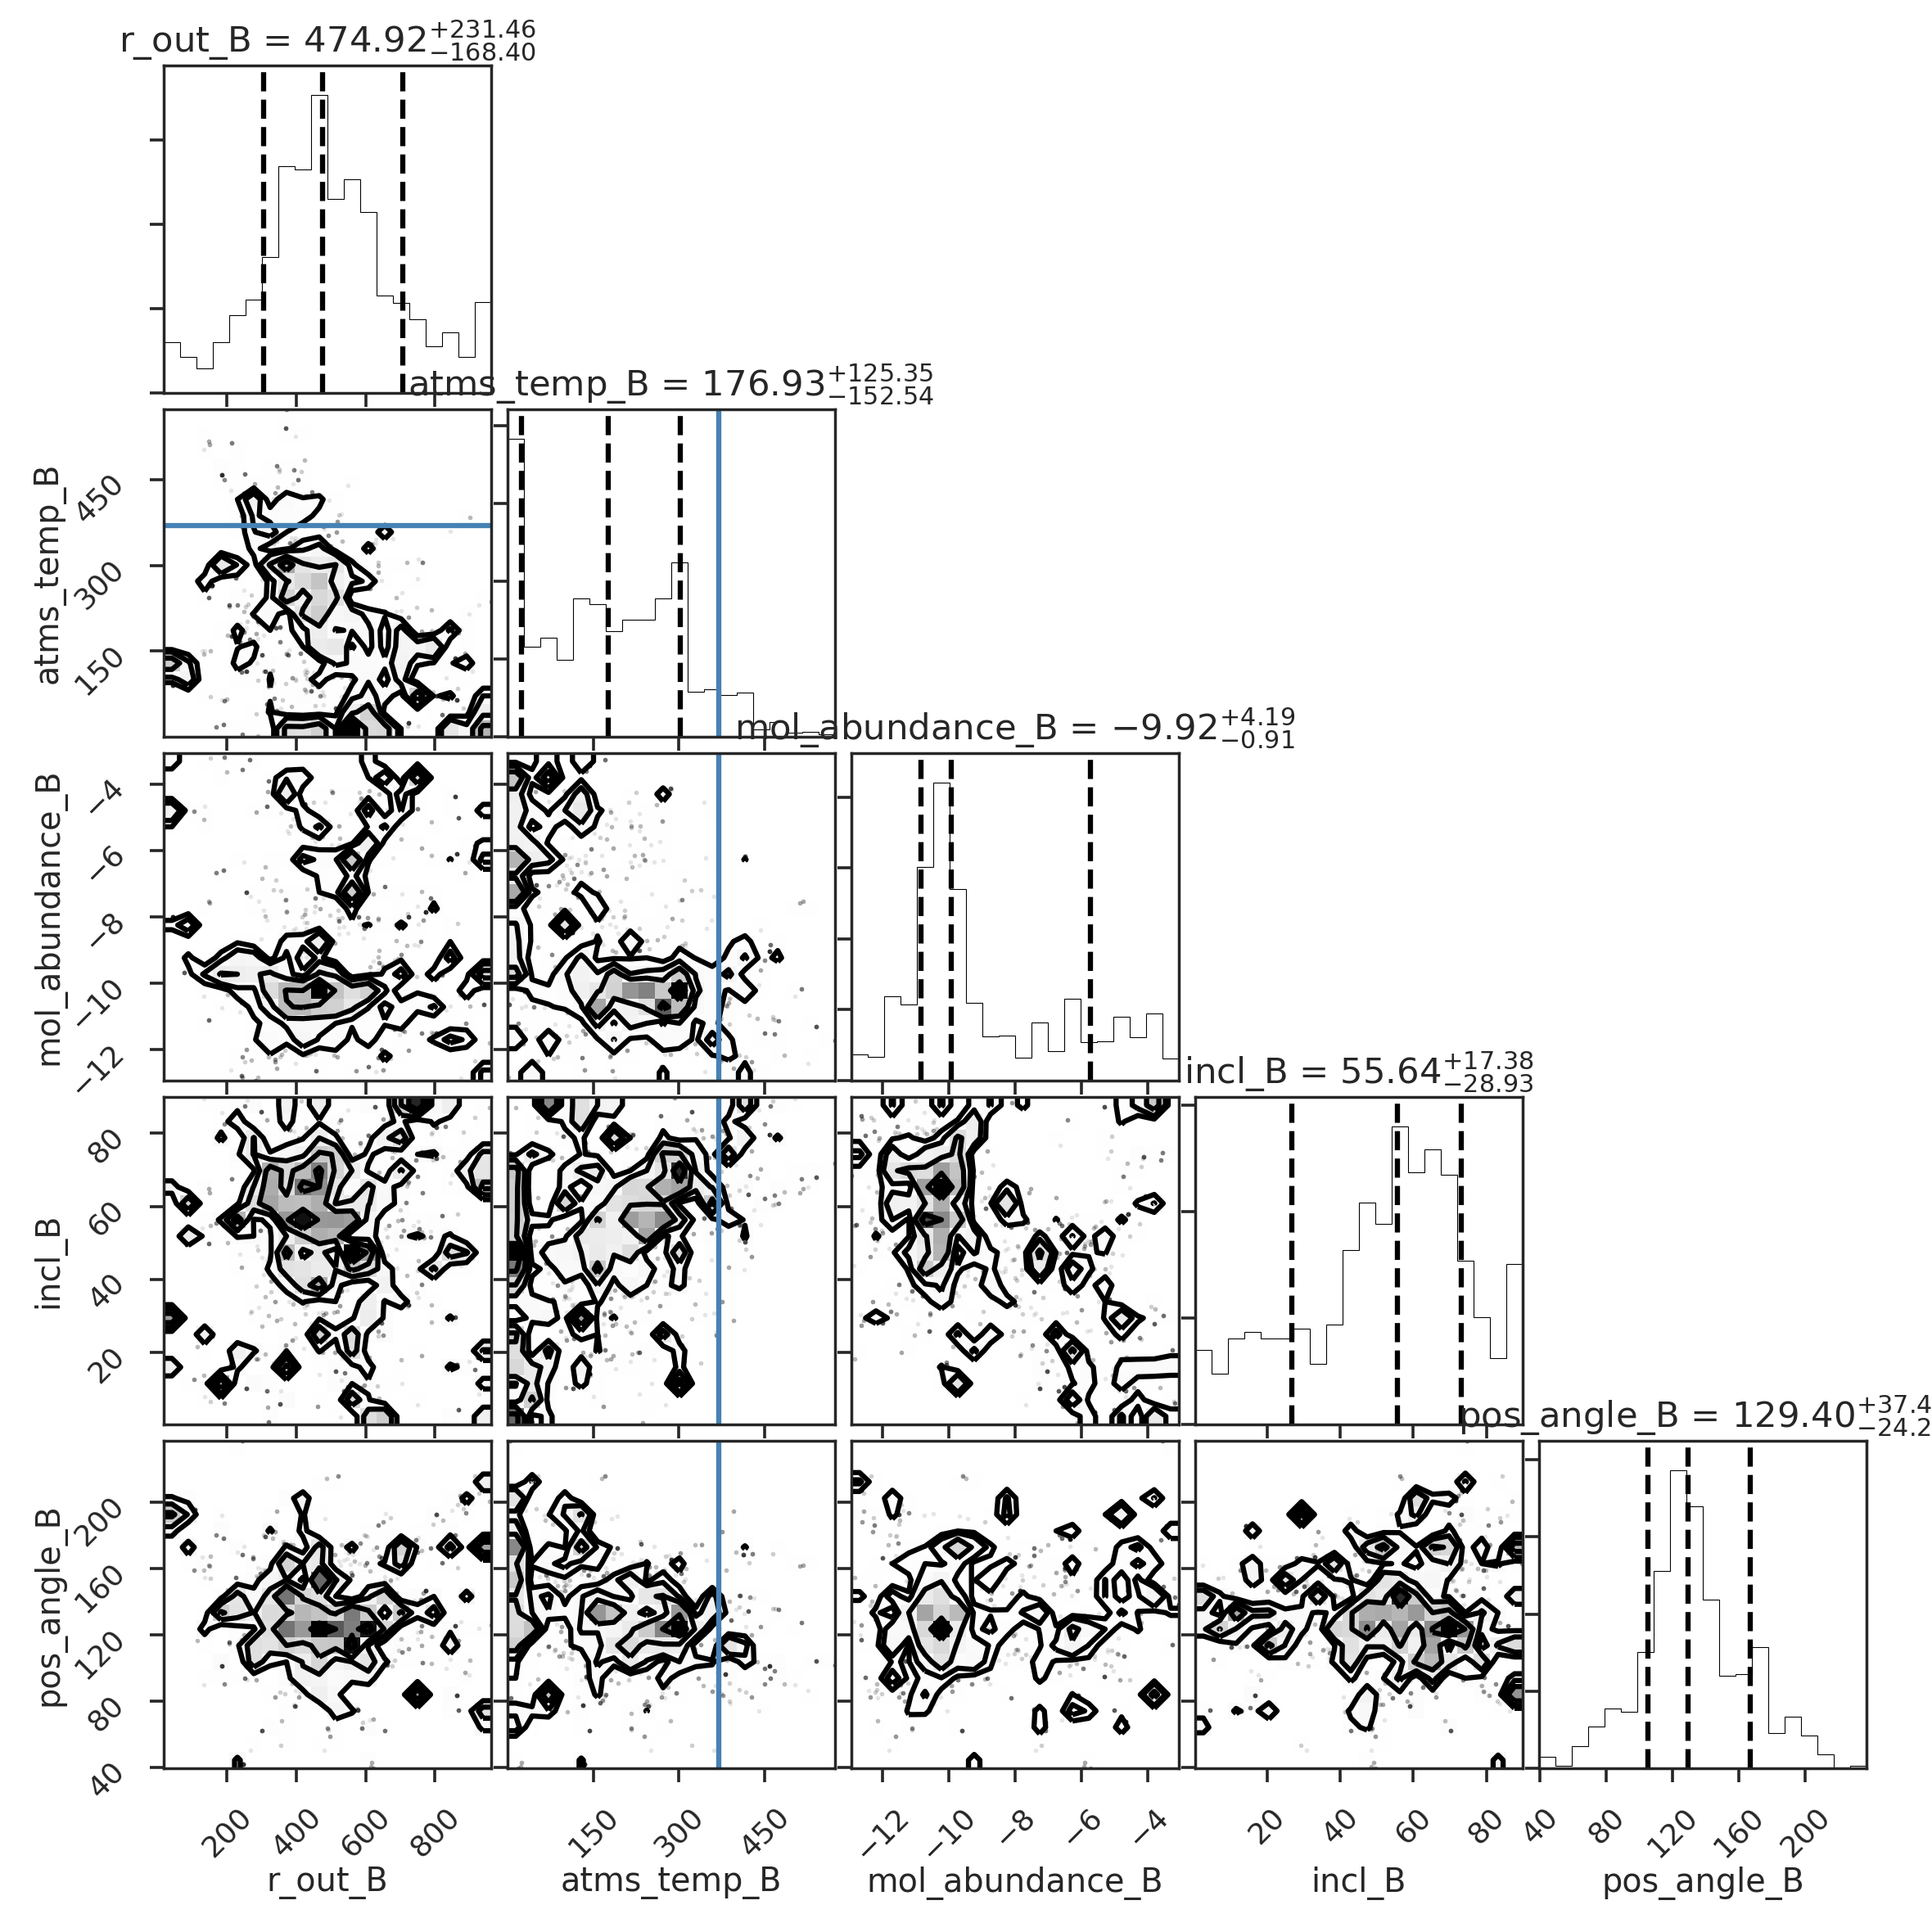
\includegraphics[width=0.49\linewidth]{cornerplot-diskB.png}}%
  \hspace*{\fill}%
  \caption{Since disk A and B's features are assumed to be independent, we may generate corner plots for each of their parameter spaces individually. Some analysis. REWORK: these are not the most recent ones}
  \label{fig:corner_plots}
\end{figure}





\section{Fitting Procedure}
\label{section:fitting_procedure}

Fitting of the data began with the analysis and partial removal of cloud contamination discussed in \S\ref{chap:results}, resulting in the removal of baselines below a characteristic length for each line. With the data as clean as possible, position ($\Delta \alpha, \Delta \delta$) and velocity ($v_\text{sys}$) offsets were fit for. Offset fitting was executed only in the HCO$^+$ line, thanks to the line's minimal contamination and high signal strength, and was performed as described in \S\ref{subsection:grid_search}. With these values established, they were treated as fixed parameters for the remainder of the fitting process.


Table \ref{table:fixed_params} presents a list of parameters, including $\Delta \alpha, \Delta \delta$, and $v_\text{sys}$, which were left fixed throughout the MCMC runs. Since we are only modeling one line at a time, we are unable to constrain the vertical temperature structure and so fix T$_\text{mid}$ and $z_q$. The selection of T$_\text{mid}$ was made following \citet{Factor2017} to reflect the ``CO snow line" shown by \citet{Qi2011}\footnote{Although their measurements were made for sources in a different environment, the value gives us a reasonable starting point for our fits.}, while the value of $z_q$ was chosen, again following \citet{Factor2017}, to be roughly double the disks' scale heights, as shown in \citet{Rosenfeld2013}. Since \hco is optically thin, temperature and density are degenerate, so $\gamma$ is set at 1 following \cite{Andrews2009}, who showed this to be a reasonable value for disks in $\rho$ Ophiuchus. Since our observations do not have enough spectral resolution to constrain the observations' turbulent linewidth, we fix $v_{turb}$ at around 1\% of the sound speed, per \citet{Flaherty2015}.

When fitting CO, we fix its abundance at the canonical value of 10$^{-4}$ and instead fit for disk mass. Conversely, in our fits of \hco and HCN emission, we fix M$_\text{disk}$ at values drawn from \cite{Williams2014}, which they infer from continuum flux measurements (and relying on the 100:1 gas/dust ratio discussed in \S\ref{chap:introduction}). The remaining parameters are fit for using MCMC. We implement priors on each parameter, reported in Table \ref{table:fit_priors}. Gaussian priors are used for the fitting of both disks' position angles, centered at values reported by \cite{Williams2014}.


\begin{table}
  \begin{threeparttable}
    \centering
    \caption{Fixed Parameter Values}
    \label{table:fixed_params}
    \renewcommand{\arraystretch}{1.2}
    \begin{tabular}{l  l  l  c  c }
      \toprule \toprule
      \multirow{2}{*}{Parameter} & \multirow{2}{*}{Description} & \multirow{2}{*}{Ref.} & \multicolumn{2}{c}{Fixed Value(s)} \\
                                 &                              &                         & Disk A & Disk B \\
      \midrule %\midrule
      $\Delta \alpha$ ($''$)       &  RA offset from image center     & 0  & 0.0002 & -1.006  \\
      $\Delta \delta$ ($''$)       &  Dec offset from image center    & 0  & 0.082  & -0.3    \\
      v$_\text{sys}$ (km s$^{-1}$) &  Systemic velocity               & 0  & 10.00  & 10.75   \\
      $i$ ($^o$)                   &  Inclination                     & 1  & 65     & 45      \\
      M$_\star$ (M$_\odot$)        &  Stellar mass                    & 1  & 3.5    & 0.4     \\
      Log M$_\text{disk}$ (M$_\odot$) & Disk gas mass\tnote{*}        & 1  & -1.11  & -1.55   \\
      v$_\text{turb}$ (km s$^{-1}$) &  Turbulence velocity            & 2  & \multicolumn{2}{c}{0.081}   \\
      $d$ (pc)                     &  Distance                        & 3  & \multicolumn{2}{c}{389}   \\
      R$_c$ (au)                   &  Critical radius                 & 1  & \multicolumn{2}{c}{100}\\
      $\gamma$                     &  Radial density power law index  & 4  & \multicolumn{2}{c}{1}\\
      $z_q$ (au)                   &  Disk scale height at 150 AU     & 5  & \multicolumn{2}{c}{29}\\
      T$_\text{mid}$ (K)           &  Midplane temp. at 150 AU        & 6  & \multicolumn{2}{c}{19}\\
      \bottomrule
    \end{tabular}

    \begin{tablenotes}\footnotesize
      \item[*] M$_\text{disk}$ is fixed in our fitting of \hco and HCN, and varied for CO.
      \item[0] Grid-search and/or elliptical fitting, as described in \S\ref{subsection:grid_search}
      \item[1] \citet{Williams2014}
      \item[2] \citet{Flaherty2015}
      \item[3] \citet{GaiaCollaboration2018}
      \item[4] \citet{Andrews2009}
      \item[5] \citet{Factor2017}
      \item[6] \citet{Qi2011}
    \end{tablenotes}
  \end{threeparttable}
\end{table}


\begin{table}
  \centering
  \begin{threeparttable}
    \caption{Fit Parameter Values}
    \label{table:fit_priors}
    \renewcommand{\arraystretch}{1.2}
    \begin{tabular}{l  l l }
      \toprule \toprule
      Parameter             &  Description                                     & Prior   \\
      \midrule %\midrule
      log X$_\text{mol}$    &  Molecular abundance, relative to H$_2$\tnote{a} & Log Uniform \\
      $q$                   &  Radial temperature power law index              & Uniform \\
      PA (\degree)          &  Position Angle\tnote{b}                         & Gaussian \\
      T$_\text{atms}$ (K)   & Atmosopheric temperature at 150 AU               & Uniform \\
      Log M$_\text{Disk}$ (M$_\odot$) &   Disk gas mass\tnote{*}               & Log Uniform \\
      \bottomrule
    \end{tabular}

    \begin{tablenotes}\footnotesize
      \item[a] For the CO line, X$_\text{mol}$ is fixed at the literature value of $10^{-4}$.
      \item[b] In our CO fit, disk B's position angle, PA, is fixed at the best-fit value from the \hco fits.
      \item[b] For \hco and HCN, disk mass was fixed at values from \cite{Williams2014}.
    \end{tablenotes}
  \end{threeparttable}
\end{table}


The results from the MCMC runs are presented below. To facilitate easier reading, accompanying figures are found at the end of the chapter.




\subsection{\hco (4-3) Fit}
\label{subsection:hco_fit}

We began by fitting the \hco line, using the MCMC methods explained above. Best fit and median values with 1$\sigma$ uncertainties are given in Table \ref{table:fit_hco}, while corner plots, showing the posterior distributions of the individual line fit, is shown in Fig. \ref{fig:hco_cornerplots}.


We see from the corner plots that, in general, the fits are quite well constrained. Uncertainties surrounding disk B's outer radius lead to some degeneracies, but overall this fit seems to be well managed. Inspection of the channel maps of the \hco data, best-fit model, and residuals (Fig. \ref{fig:hco_chanmaps}) show that, while the model seems to reporoduce the data's morphological structure fairly well, fluxes are systematically low, leaving significant residuals.

% REWORK: Don't forget to add in the most recent values for this.
\begin{table}[h!]
  \centering
  \begin{threeparttable}
    \caption{MCMC Fitting Results (\hco)}
    \label{table:fit_hco}
    \renewcommand{\arraystretch}{1.2}
    \begin{tabular}{l c l c l }
      \toprule \toprule
      %\multirow{2}{*}{Parameter} & \multirow{2}{*}{Disk A}    & \multicolumn{2}{c}{Disk B} \\
      \multirow{2}{*}{Parameter} & \multicolumn{2}{c}{Disk A} & \multicolumn{2}{c}{Disk B} \\
                                 & Median & Best Fit            & Median & Best Fit \\
      \midrule %\midrule
      R$_\text{out}$(au)       & $338.83_{-8.} ^{+10}$     & $342.22$ & $ 268.17_{-88.} ^{+84.}$  & $155.48$    \\
      T$_\text{atms}$ (K) & $ 221.99_{-61} ^{+109.}$  & $209.48$ & $ 182.09_{-115} ^{+66.}$  & $284.81$  \\
      X$_{\hco}$          & $ -8.40_{-0.24} ^{+0.38}$ & $-8.36$  & $ 10.32_{-0.27} ^{+0.32}$ & $-9.91$ \\
      PA  (\degree)       & $ 69.76_{-1.24} ^{+1.76}$ & $70.17$  & $ 131.86_{-14.35.} ^{+10.97}$  & $120.25$  \\
      q                   & $ 0.73_{-0.47} ^{+0.32}$  & $0.75$   & $[-0.5]$                  & $[-0.5]$  \\
      lnprob              & \multicolumn{4}{c}{$-28402$} \\
      \bottomrule
    \end{tabular}
    \begin{tablenotes}\footnotesize
      \item[*] Values in [brackets] were fixed for this run.
    \end{tablenotes}
  \end{threeparttable}
\end{table}








\subsection{HCN(4-3) Fit}
\label{subsection:hcn_fit}

Next we model HCN, using the same methods as for \hco. As before, best fit and median values with 1$\sigma$ uncertainties are given in Table \ref{table:fit_hcn}, corner plots are shown in Fig. \ref{fig:hcn_cornerplots}, and channel maps are presented in Fig. \ref{fig:hcn_chanmaps}.

In the channel maps, we see that the fit is generally good, leaving fairly minimal residuals behind. The residuals do, however, highlight a stream of flux connecting the two disks, particularly at velocities around 9.4-10.2 \kms that our model is unable to fit. This stream is most visible in the HCN line, compared to the \hco and CO maps.

For both disks, the posterior distribution of fits to outer radius is bimodal. This likely is a result of the MCMC walkers struggling to make sense of the above-mentioned bridge between the disks. This is particularly the case with disk B, where the walkers are distributed around 100 AU and around 350 AU. As a test, we can remove all steps in the MCMC chain where disk B's outer radius exceeds 220 AU (which is somewhere in the middle of the bimodality in the parameter's posterior distribution, but is still appreciably higher than the \hco fit value of $\sim$150 AU). Doing so brings \hco and HCN into almost perfect agreement (\textless 1\%) on disk B's outer radius, while also increasing disk A's HCN abundance by more than an order of magnitude and pushing disk B's temperature up to more than twice the value found for the \hco line. See Table \ref{tab:hcn_short_rout} for a selection of the fit parameters, selected based on whether they change with the radius cut. As a visual check on whether this yields a better fit, Fig \ref{fig:hcn_m1_ellipses} shows HCN's first moment map with both best-fit disk B radii plotted.

Otherwise, the fit's posteriors are widely unimodal and less tightly constrained than those from the \hco fits. There are no particularly noticeable degeneracies between parameters.



% Note: Maybe use pd.df.to_latex() to populate these tables?
\begin{table}[h!]
  \centering
  \begin{threeparttable}
    \caption{MCMC Fitting Results (HCN)}
    \label{table:fit_hcn}
    \renewcommand{\arraystretch}{1.2}
    \begin{tabular}{l c l c l }
      \toprule \toprule
      %\multirow{2}{*}{Parameter} & \multirow{2}{*}{Disk A}    & \multicolumn{2}{c}{Disk B} \\
      \multirow{2}{*}{Parameter} & \multicolumn{2}{c}{Disk A} & \multicolumn{2}{c}{Disk B} \\
                                 & Median & Best Fit          & Median & Best Fit \\
      \midrule %\midrule
      R$_\text{out}$ (au)      & $ 448.23_{-120.17} ^{+146.62}$ & $334.68$ & $ 217.02_{-152.70}^{+133.53}$   & $324.50$  \\
      T$_\text{atms}$ (K) & $ 169.06_{-95.87} ^{+166.57}$  & $140.95$ & $ 155.78_{-106.03} ^{+188.93.}$ & $205.85$  \\
      X$_{HCN}$           & $ -9.01_{-0.55} ^{+0.89}$      & $-7.62$  & $ 10.81_{-1.32} ^{+0.95}$       & $-10.55$  \\
      PA (\degree)        & $ 69.89_{-1.81} ^{+1.64}$      & $69.30$  & $ -134.77_{-18.61} ^{+16.15}$   & $132.22$  \\
      q                   & $ 0.87_{-0.59} ^{+0.59}$       & $0.72$   & $[-0.5]$                        & $[-0.5]$  \\
      $\ln$ Likelihood    & \multicolumn{4}{c}{$-30928.13$} \\
      \bottomrule
    \end{tabular}
    \begin{tablenotes}\footnotesize
      \item[*] Values in [brackets] were fixed for this run.
    \end{tablenotes}
  \end{threeparttable}
\end{table}



\begin{table}
  \centering
  \begin{threeparttable}
    \caption{HCN Fits, R$_\text{out, B}$ \textless 220}
    \label{table:hcn_short_rout}
    \renewcommand{\arraystretch}{1.2}
    \begin{tabular}{l c c c c }
      \toprule \toprule
      %\multirow{2}{*}{Parameter} & \multirow{2}{*}{Disk A}    & \multicolumn{2}{c}{Disk B} \\
                & X$_\text{mol}$ & R$_\text{out}$ (au)     & $q$    & T$_\text{atms}$ (K) \\
      \midrule %\midrule
        Disk A  & -6.98          & 337.57             & 0.89   & 86.13 \\
        Disk B  & -10.3          & 145.57             & [-0.5] & 281.89 \\
      \bottomrule
    \end{tabular}
    % \begin{tablenotes}\footnotesize
    % \end{tablenotes}
  \end{threeparttable}
\end{table}




\subsection{CO(3-2) Fit}
\label{subsection:co_fit}
Finally, we fit the CO(3-2) line. Despite the removal of baselines below 60 k$\lambda$, the CO(3-2) line still shows significant cloud contamination in channels near the systemic velocity (Fig. \ref{fig:co_chanmaps}). In an attempt to keep the MCMC walkers from trying to fit the contamination, we did not evaluate the $\chi^2$ contribution of the channels with velocities between 9.88 and 12 \kms, which show the worst of the clouds' effects. By choosing to not include these, we sacrifice some data, but the resulting fits are more representative of the structures we care about - the disks themselves - than they would be had we not sacrificed those channels. However, since it seems that this was insufficient, it is likely that it would have been preferable to exclude a far wider range of contaminated channels, likely from around 6.5 - 13.3 \kms.


\begin{table}[h!]
  \centering
  \begin{threeparttable}
    \caption{MCMC Fitting Results (CO)}
    \label{table:fit_co}
    \renewcommand{\arraystretch}{1.2}
    \begin{tabular}{l c l c l }
      \toprule \toprule
      \multirow{2}{*}{Parameter} & \multicolumn{2}{c}{Disk A} & \multicolumn{2}{c}{Disk B} \\
                                 & Median & Best Fit          & Median & Best Fit \\
      \midrule %\midrule
      R$_\text{out}$(au)       & $ 392.66_{-114.75}^{+0.99.21}$       & $492.76$ & $ 199.45_{-68.67} ^{+83.34}$ & $133.02$ \\
      T$_\text{atms}$ (K) & $ 222.99_{-218.54} ^{+228.78}$       & $2.87 $  & $273.39_{-155.72}^{+132.27}$ & $473.20$ \\
      log M$_\text{Disk}$ (M$_\odot$) & $ -2.56_{-0.45}^{+2.03}$ & $-0.03$  & $ -4.76_{-0.44} ^{+0.36}$    & $-5.18$  \\
      PA  (\degree)       & $ 70.51_{-2.71}^{+3.05}$             & $72.28$  & $[136]$                      & $[136]$  \\
      q                   & $ -0.03_{-0.47} ^{+0.46}$            & $-0.03$  & $[-0.5]$                     & $[-0.5]$ \\
      $\ln$ Likelihood    & \multicolumn{4}{c}{$-33577.41$} \\
      \bottomrule
    \end{tabular}



    \begin{tablenotes}\footnotesize
      \item[*] Values in [brackets] were fixed for this run.
    \end{tablenotes}
  \end{threeparttable}
\end{table}

Consequentially, the resulting fits are noticeably less certain than those of the HCO+ and HCN lines, featuring several jagged and bimodal posteriors, shown in Fig.\ref{fig:co_cornerplots}. Additionally, since the best-fit values disagree significantly with the results from the other lines (particularly in the T$_\text{atms}$ for disk A, which is unrealistically low), we are unable to include these results in our analysis.

Despite this, the CO line seems to have had some marginal success in recovering disk radii, returning a best-fit value disk B that is within \textless10\% of the \hco line's reported value, and, although the best-fit radius for disk A is unreasonably high at nearly 500 AU, the model's 50$^\text{th}$ percentile fit is within 15\% of the \hco value. This seems to indicate that these data still have potential value if constrained appropriately.



Fig.\ref{fig:bf_disk_strs} show the resulting best-fit temperature and density structures in each line.








%% ~~~~ FIGURES ~~~~~~~~~~~~~~~~~~~~~~~~~~~~~~~~~~~~~~~~~~~~~~~~~~~~~~~~~~~~~~~~


%% ~~~ HCO ~~~~~~~~~~~~~~~~~~~~~~~~~~~~~~~~~~~~~~~~~~~~~~~~~~~~~~~~~~~~~~~~~~~~~


\begin{figure}[htp]
  \hspace*{\fill}%
  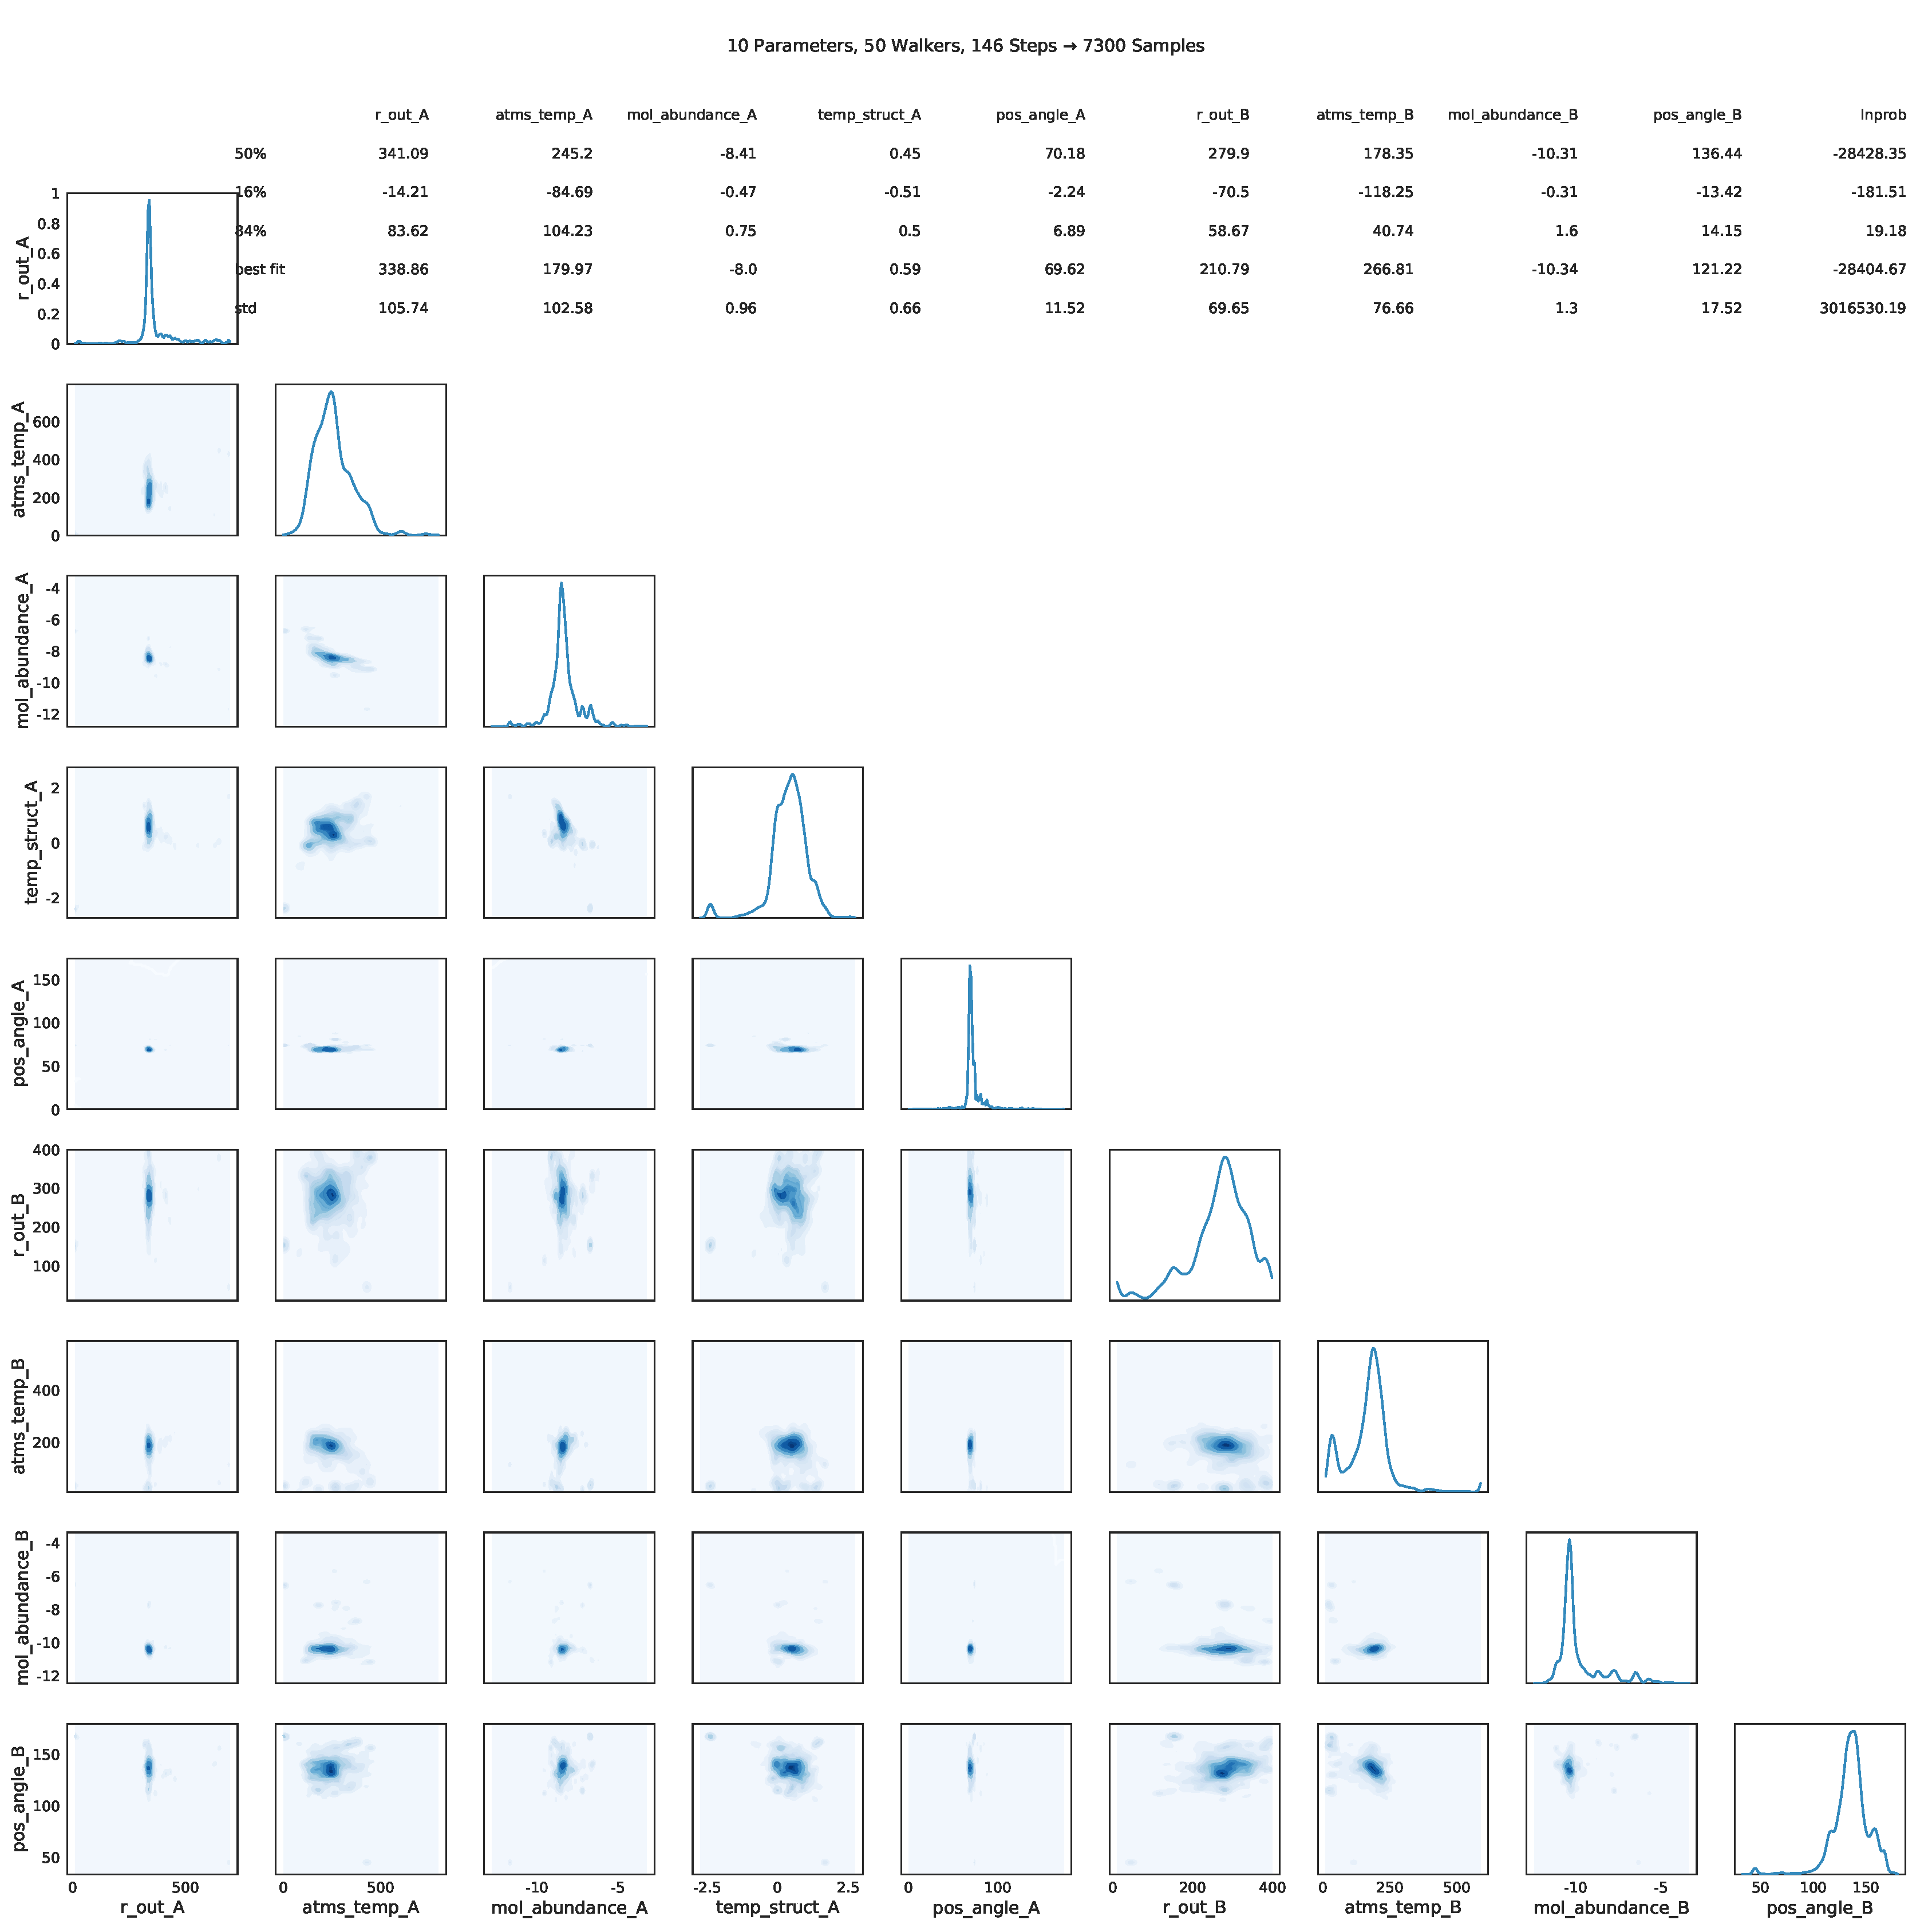
\includegraphics[width=\linewidth]{cornerplots-hco.pdf}\hfill%
  \hspace*{\fill}%
  \caption{Cornerplots of results from MCMC fitting of \hco emission.}
  \label{fig:hco_cornerplots}
\end{figure}



\begin{figure}[htp]
  \hspace*{\fill}%
  \includegraphics[width=\linewidth]{chanmaps-hco.pdf}\hfill%
  \hspace*{\fill}%
  \caption{Channel maps of \hco emission data, as well as a best-fit model from MCMC fitting and residuals from the two.}
  \label{fig:hco_chanmaps}
\end{figure}

%% ~~~ HCN ~~~~~~~~~~~~~~~~~~~~~~~~~~~~~~~~~~~~~~~~~~~~~~~~~~~~~~~~~~~~~~~~~~~~~

\begin{figure}[htp]
  \hspace*{\fill}%
  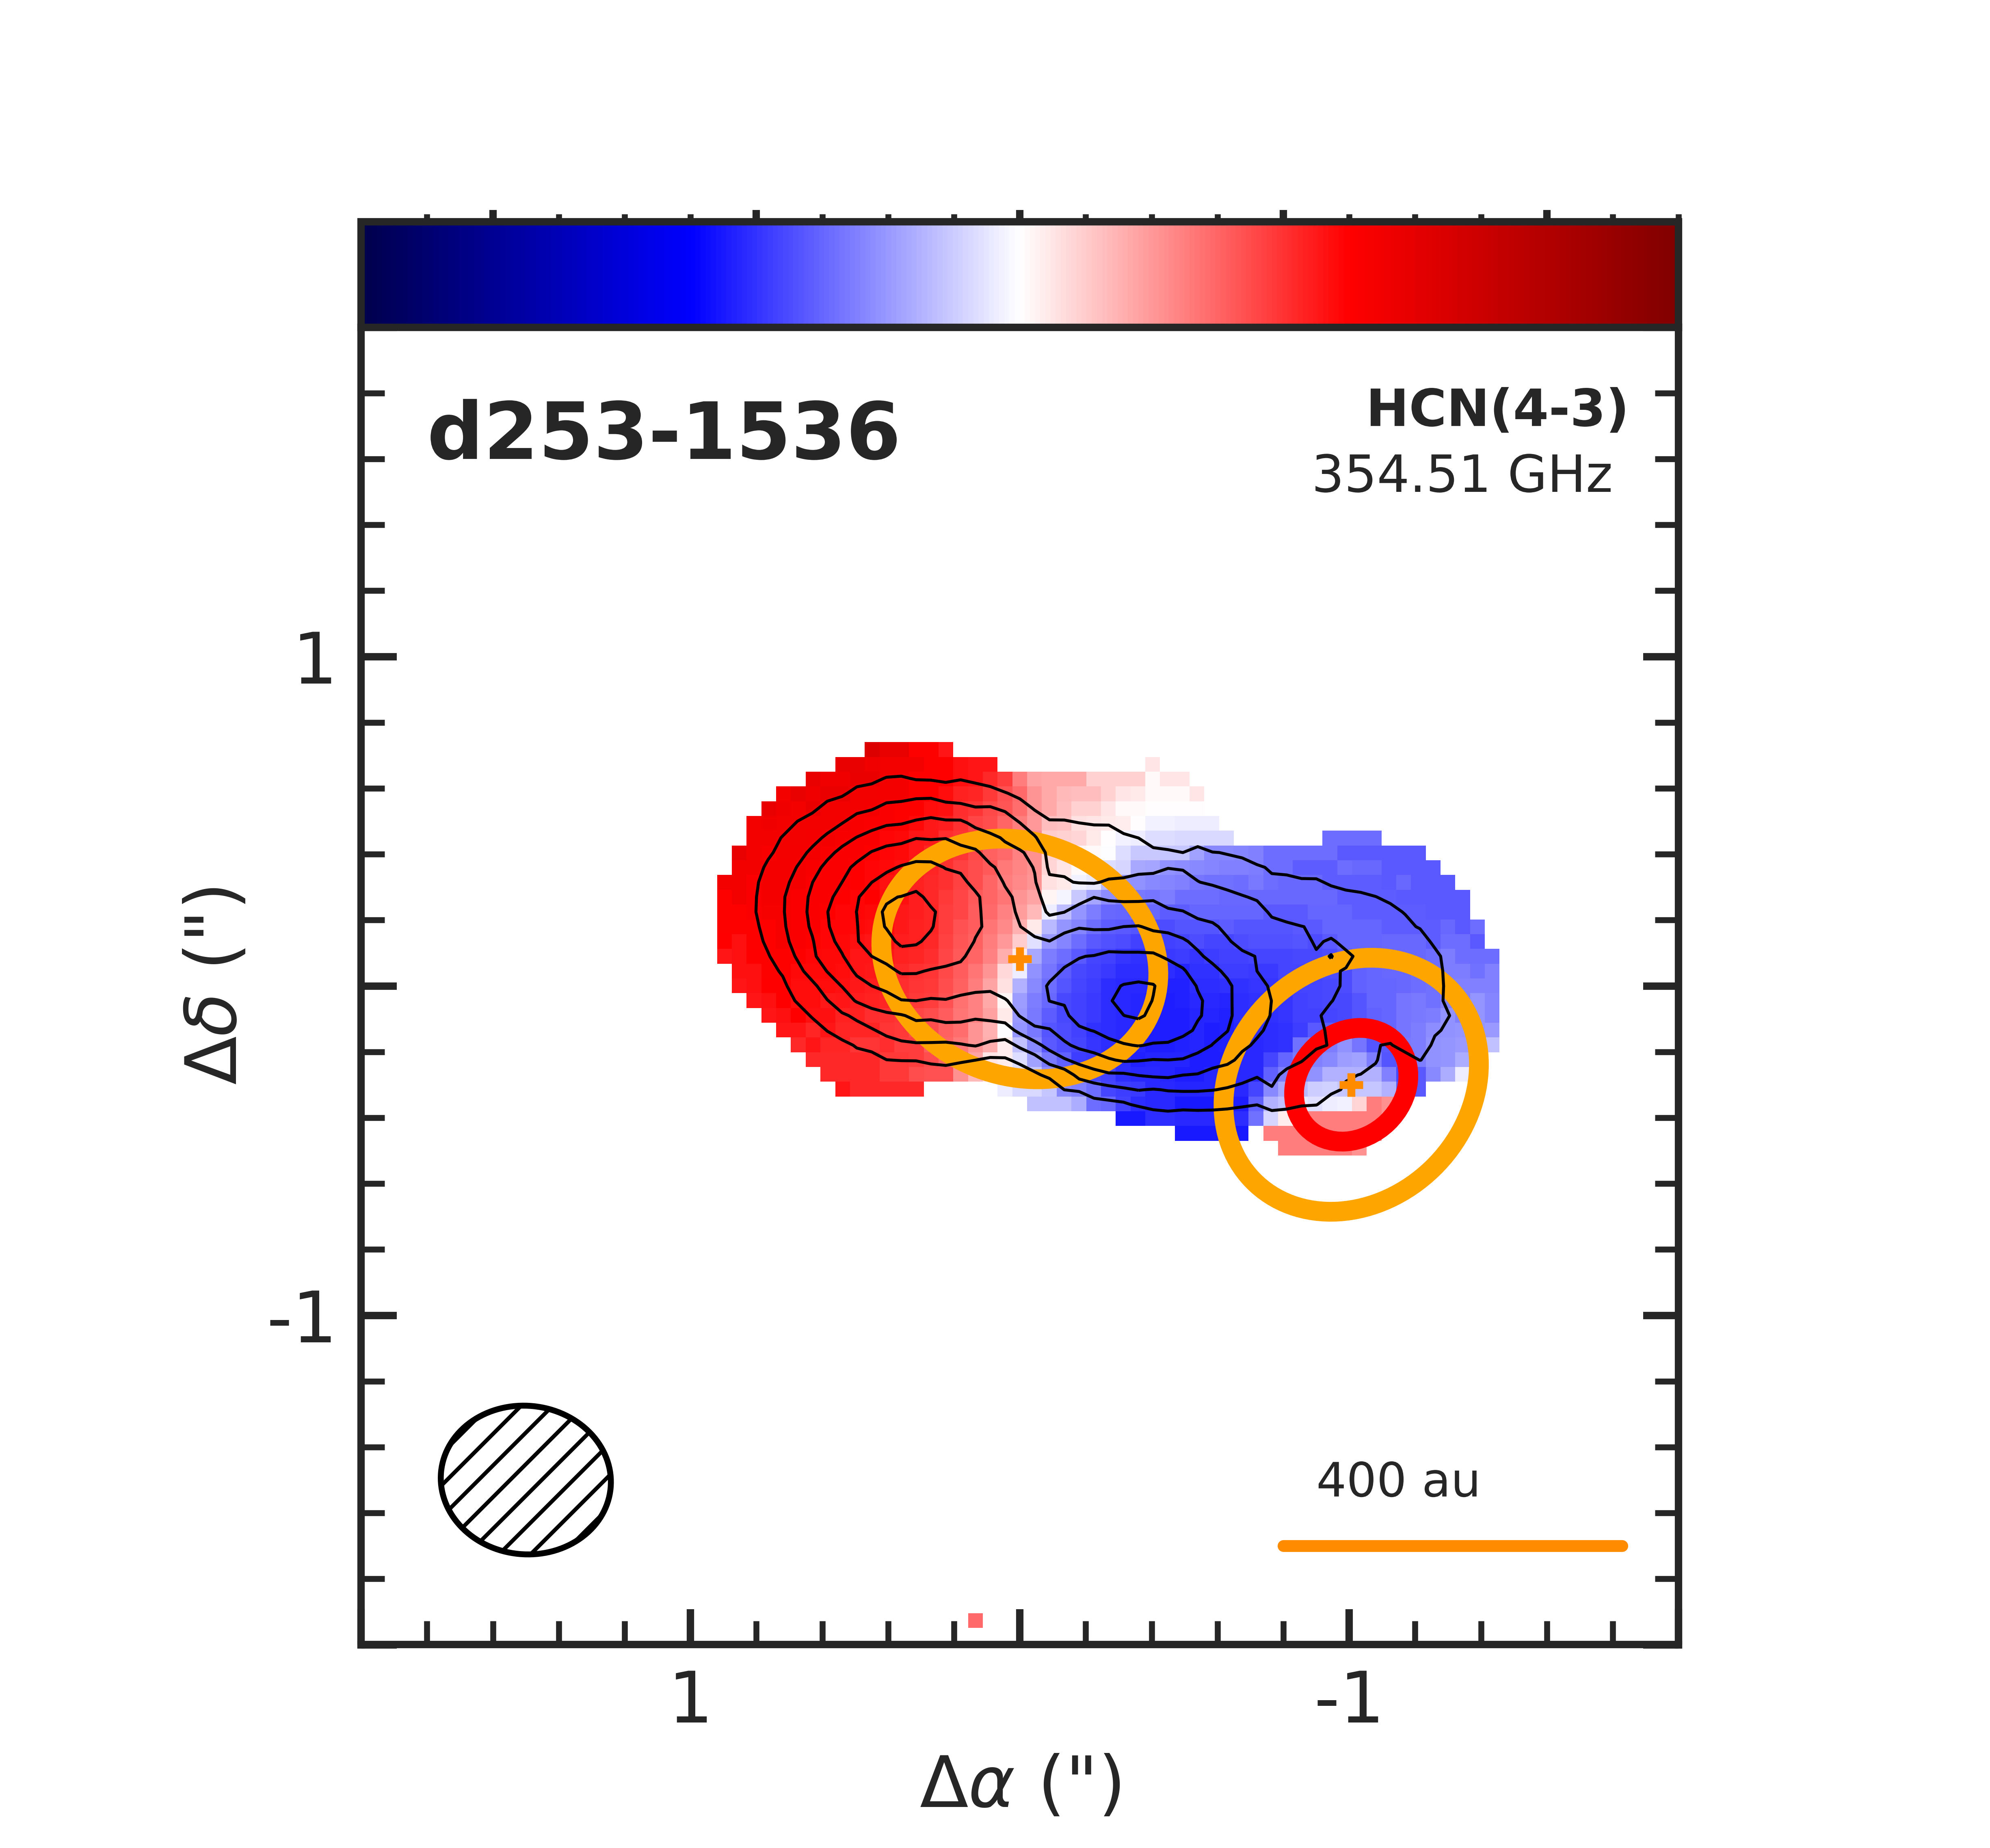
\includegraphics[width=\linewidth]{m1-map_hcn_withellipses.png}\hfill%
  \hspace*{\fill}%
  \caption{Moment-1 map of HCN emission, overlaid with ellipses described by each disk's best-fit position angle, inclination, and outer radius. For disk B, both the best-fit outer radius with and without the 220 AU a posteriori prior implemented (at 324 and 145 AU, respectively) are plotted.}
  \label{fig:hcn_m1_ellipses}
\end{figure}


\begin{figure}[htp]
  \hspace*{\fill}%
  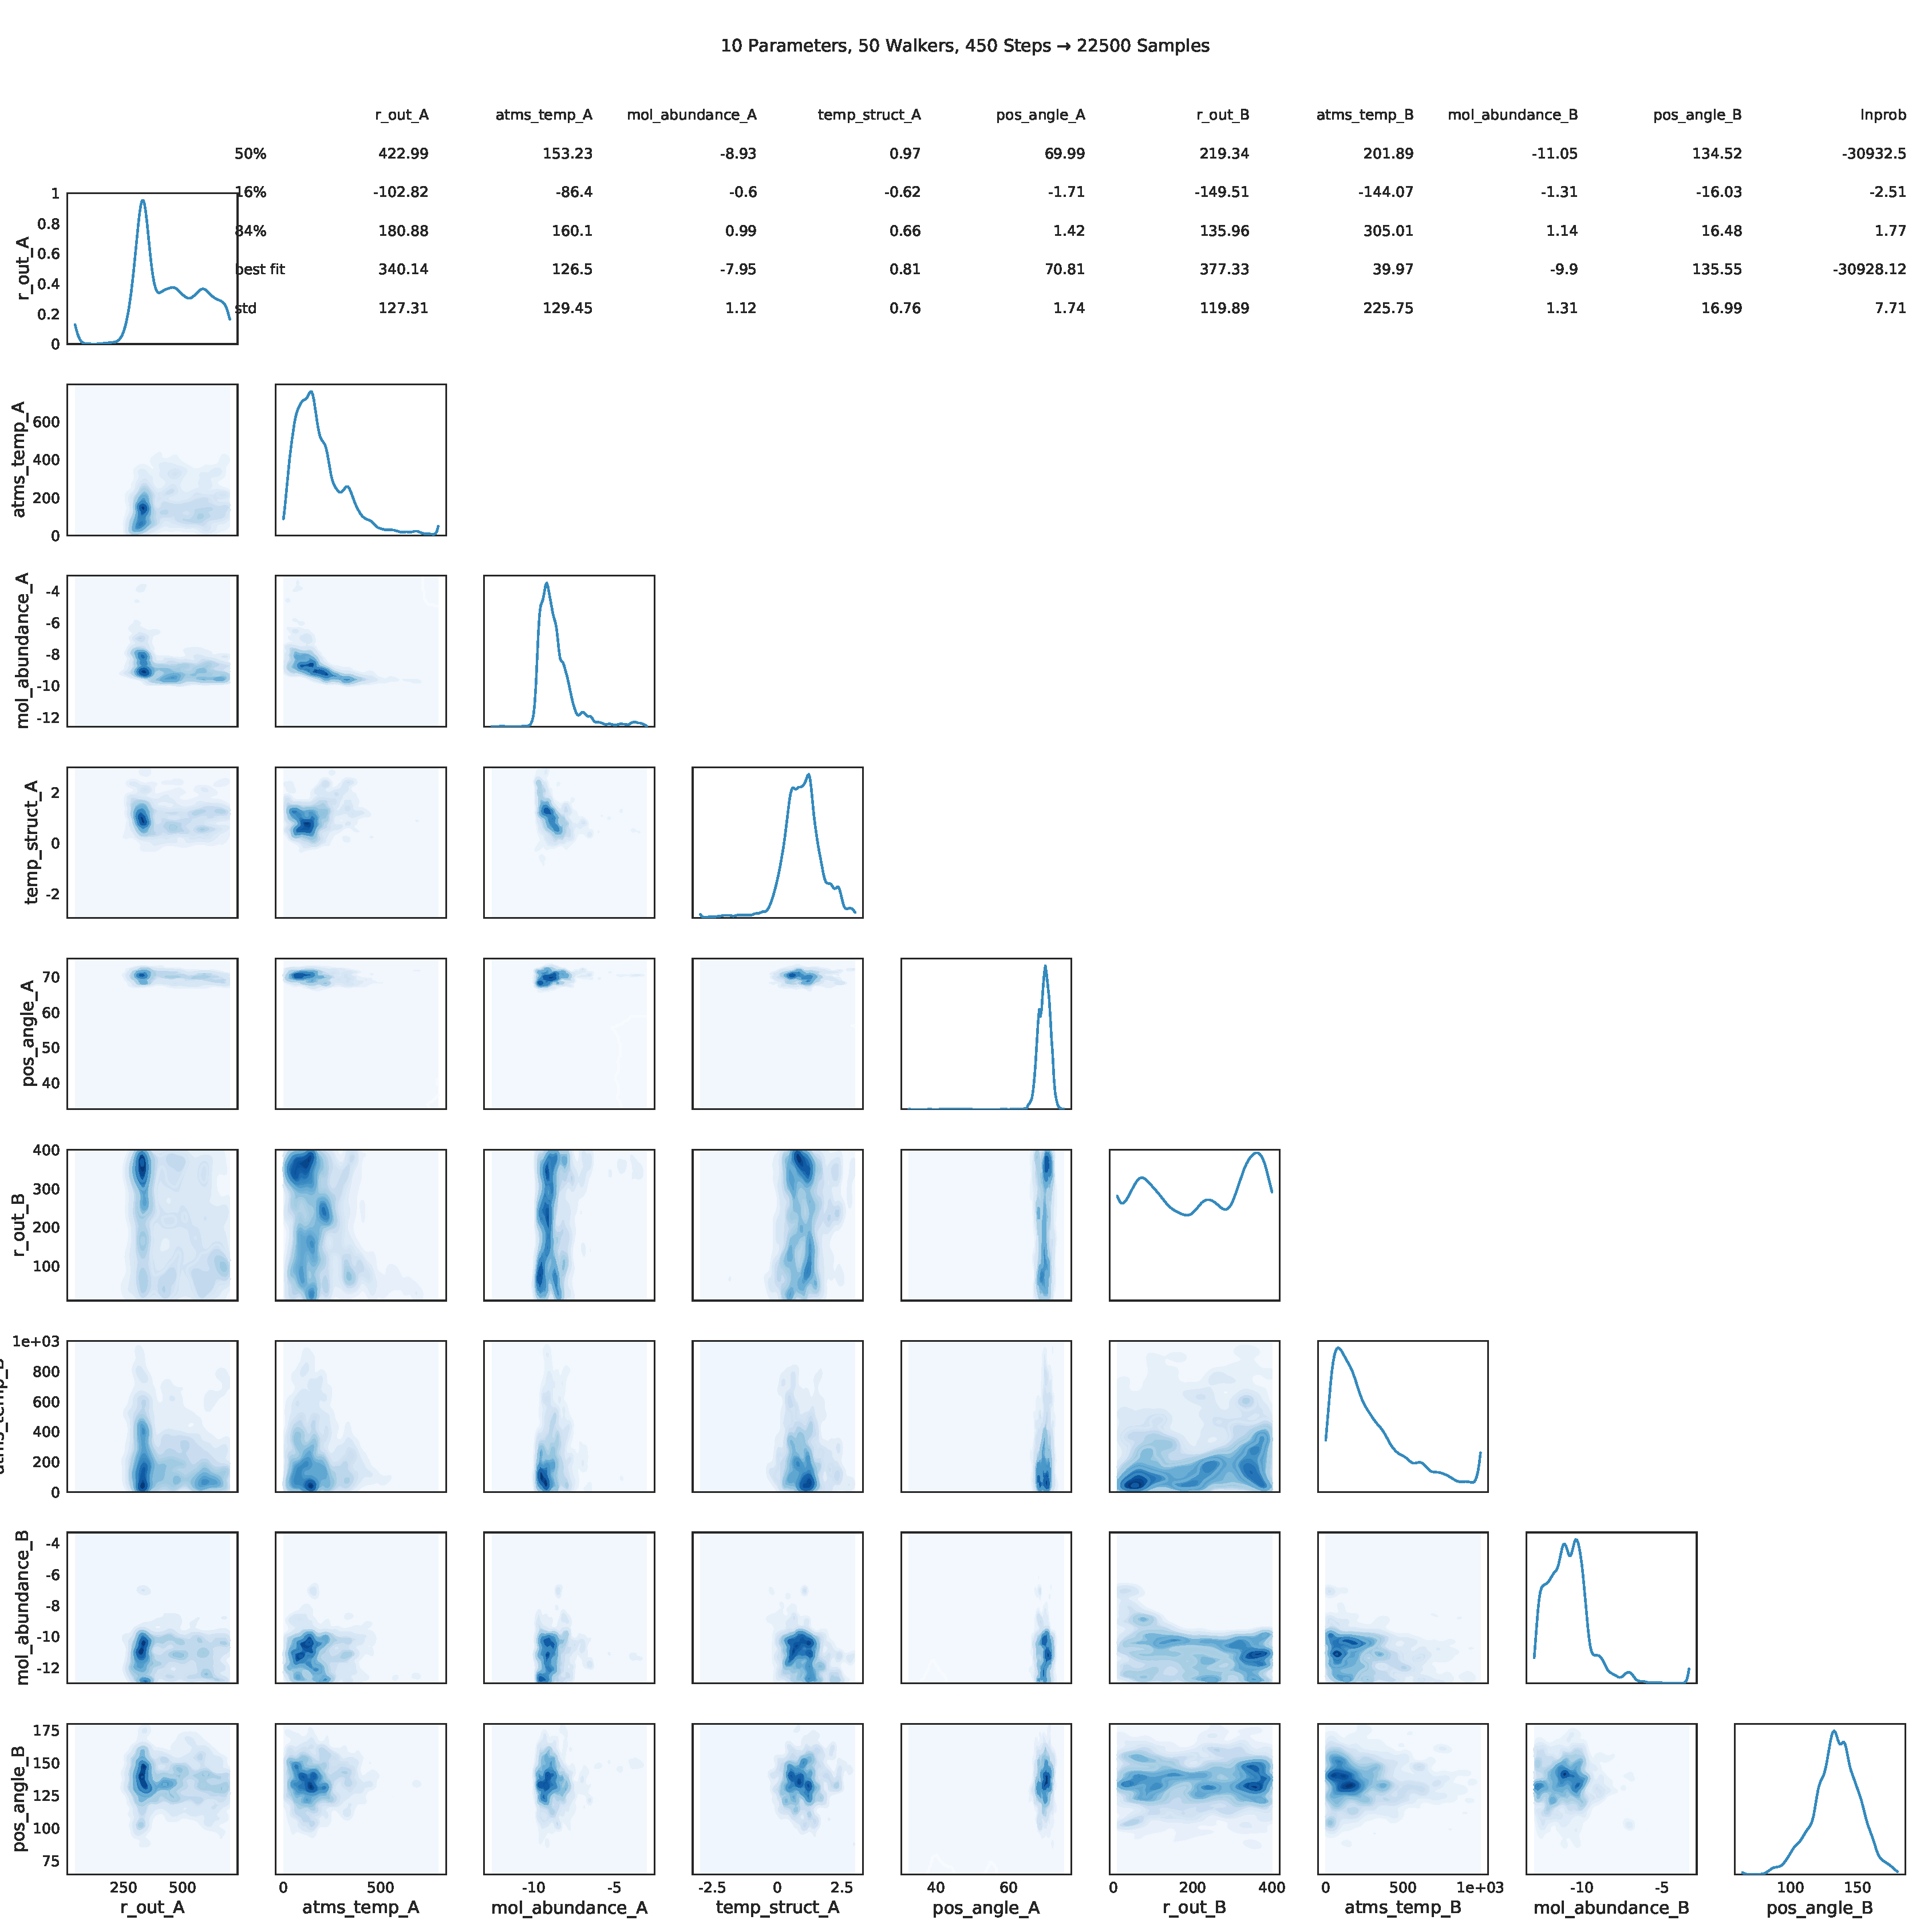
\includegraphics[width=\linewidth]{cornerplots-hcn.pdf}\hfill%
  \hspace*{\fill}%
  \caption{Cornerplots of results from MCMC fitting of HCN emission.}
  \label{fig:hcn_cornerplots}
\end{figure}



\begin{figure}[htp]
  \hspace*{\fill}%
  \includegraphics[width=\linewidth]{chanmaps-hcn.pdf}\hfill%
  \hspace*{\fill}%
  \caption{Channel maps of HCN emission data, as well as a best-fit model from MCMC fitting and residuals from the two.}
  \label{fig:hcn_chanmaps}
\end{figure}



%% ~~~ CO ~~~~~~~~~~~~~~~~~~~~~~~~~~~~~~~~~~~~~~~~~~~~~~~~~~~~~~~~~~~~~~~~~~~~~~

\begin{figure}[htp]
  \hspace*{\fill}%
  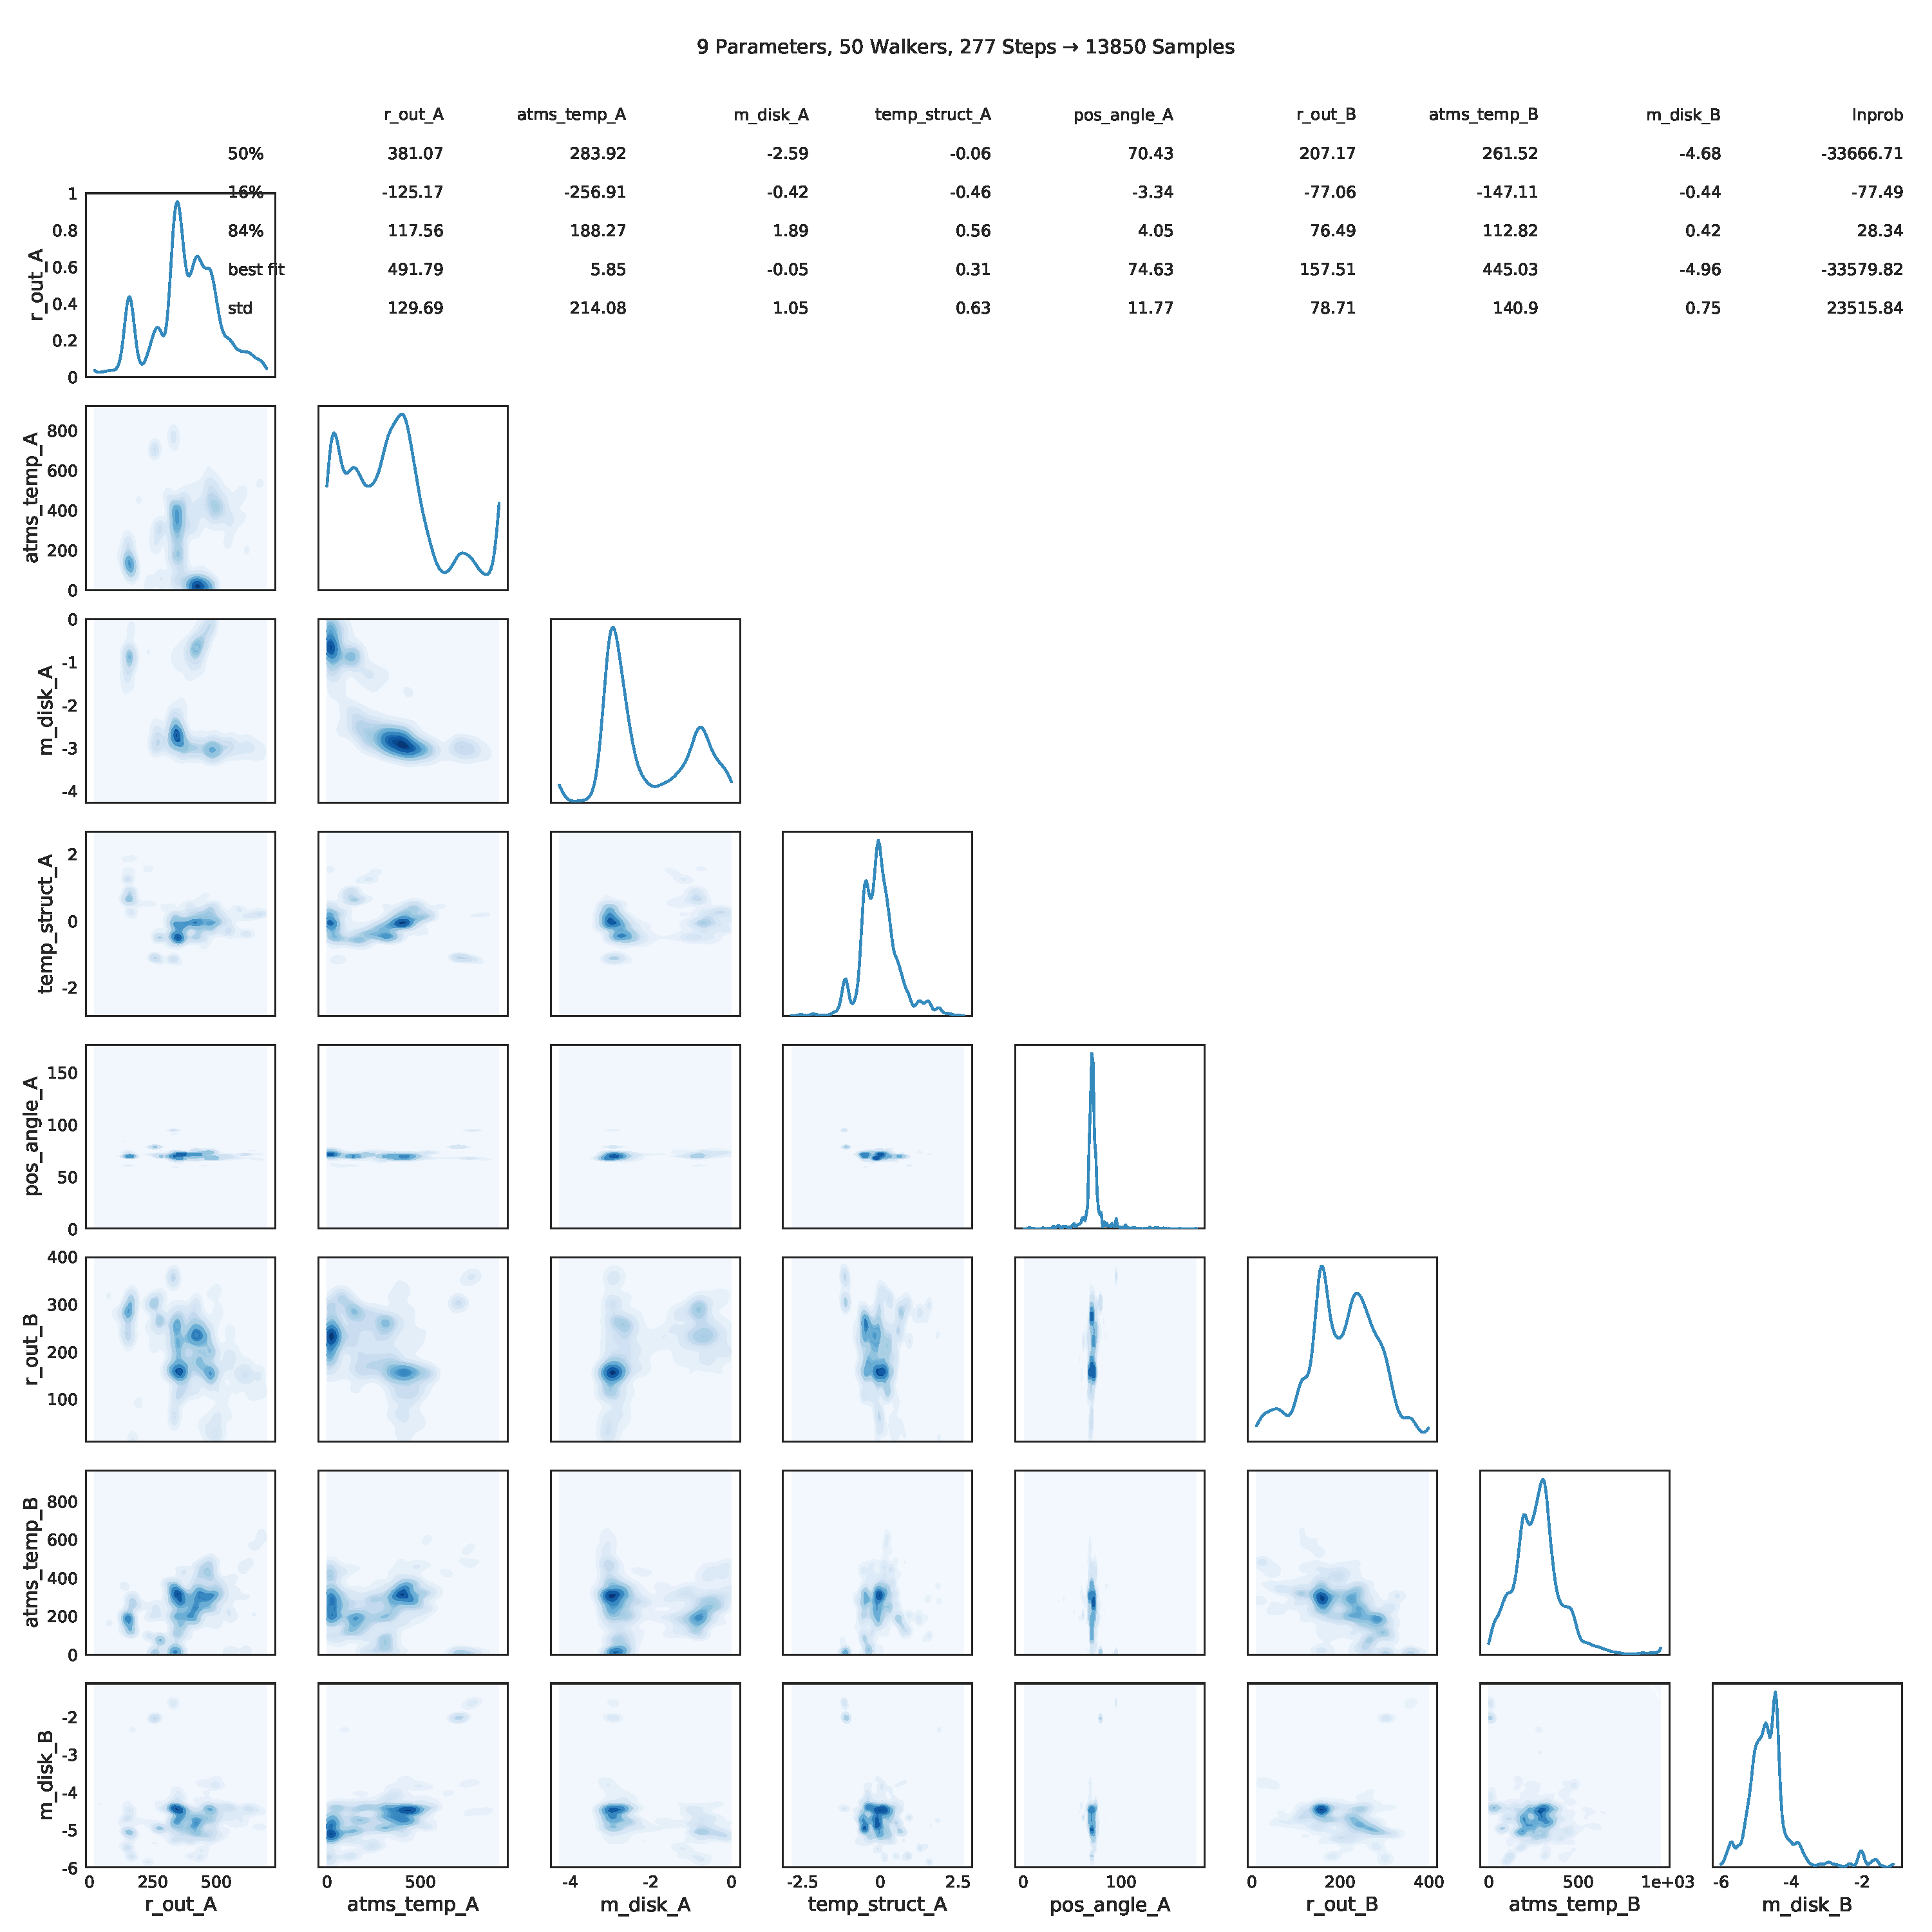
\includegraphics[width=\linewidth]{cornerplots-co.pdf}\hfill%
  \hspace*{\fill}%
  \caption{Cornerplots of results from MCMC fitting of HCN emission.}
  \label{fig:co_cornerplots}
\end{figure}


\begin{figure}[htp]
  \hspace*{\fill}%
  \includegraphics[width=\linewidth]{chanmaps-co.pdf}\hfill%
  \hspace*{\fill}%
  \caption{Channel maps of CO emission data, as well as a best-fit model from MCMC fitting and residuals from the two.}
  \label{fig:co_chanmaps}
\end{figure}




% \begin{figure}[htp]
%   \hspace*{\fill}%
%   \subcaptionbox{Disk A fits \label{fig:corner_a}}{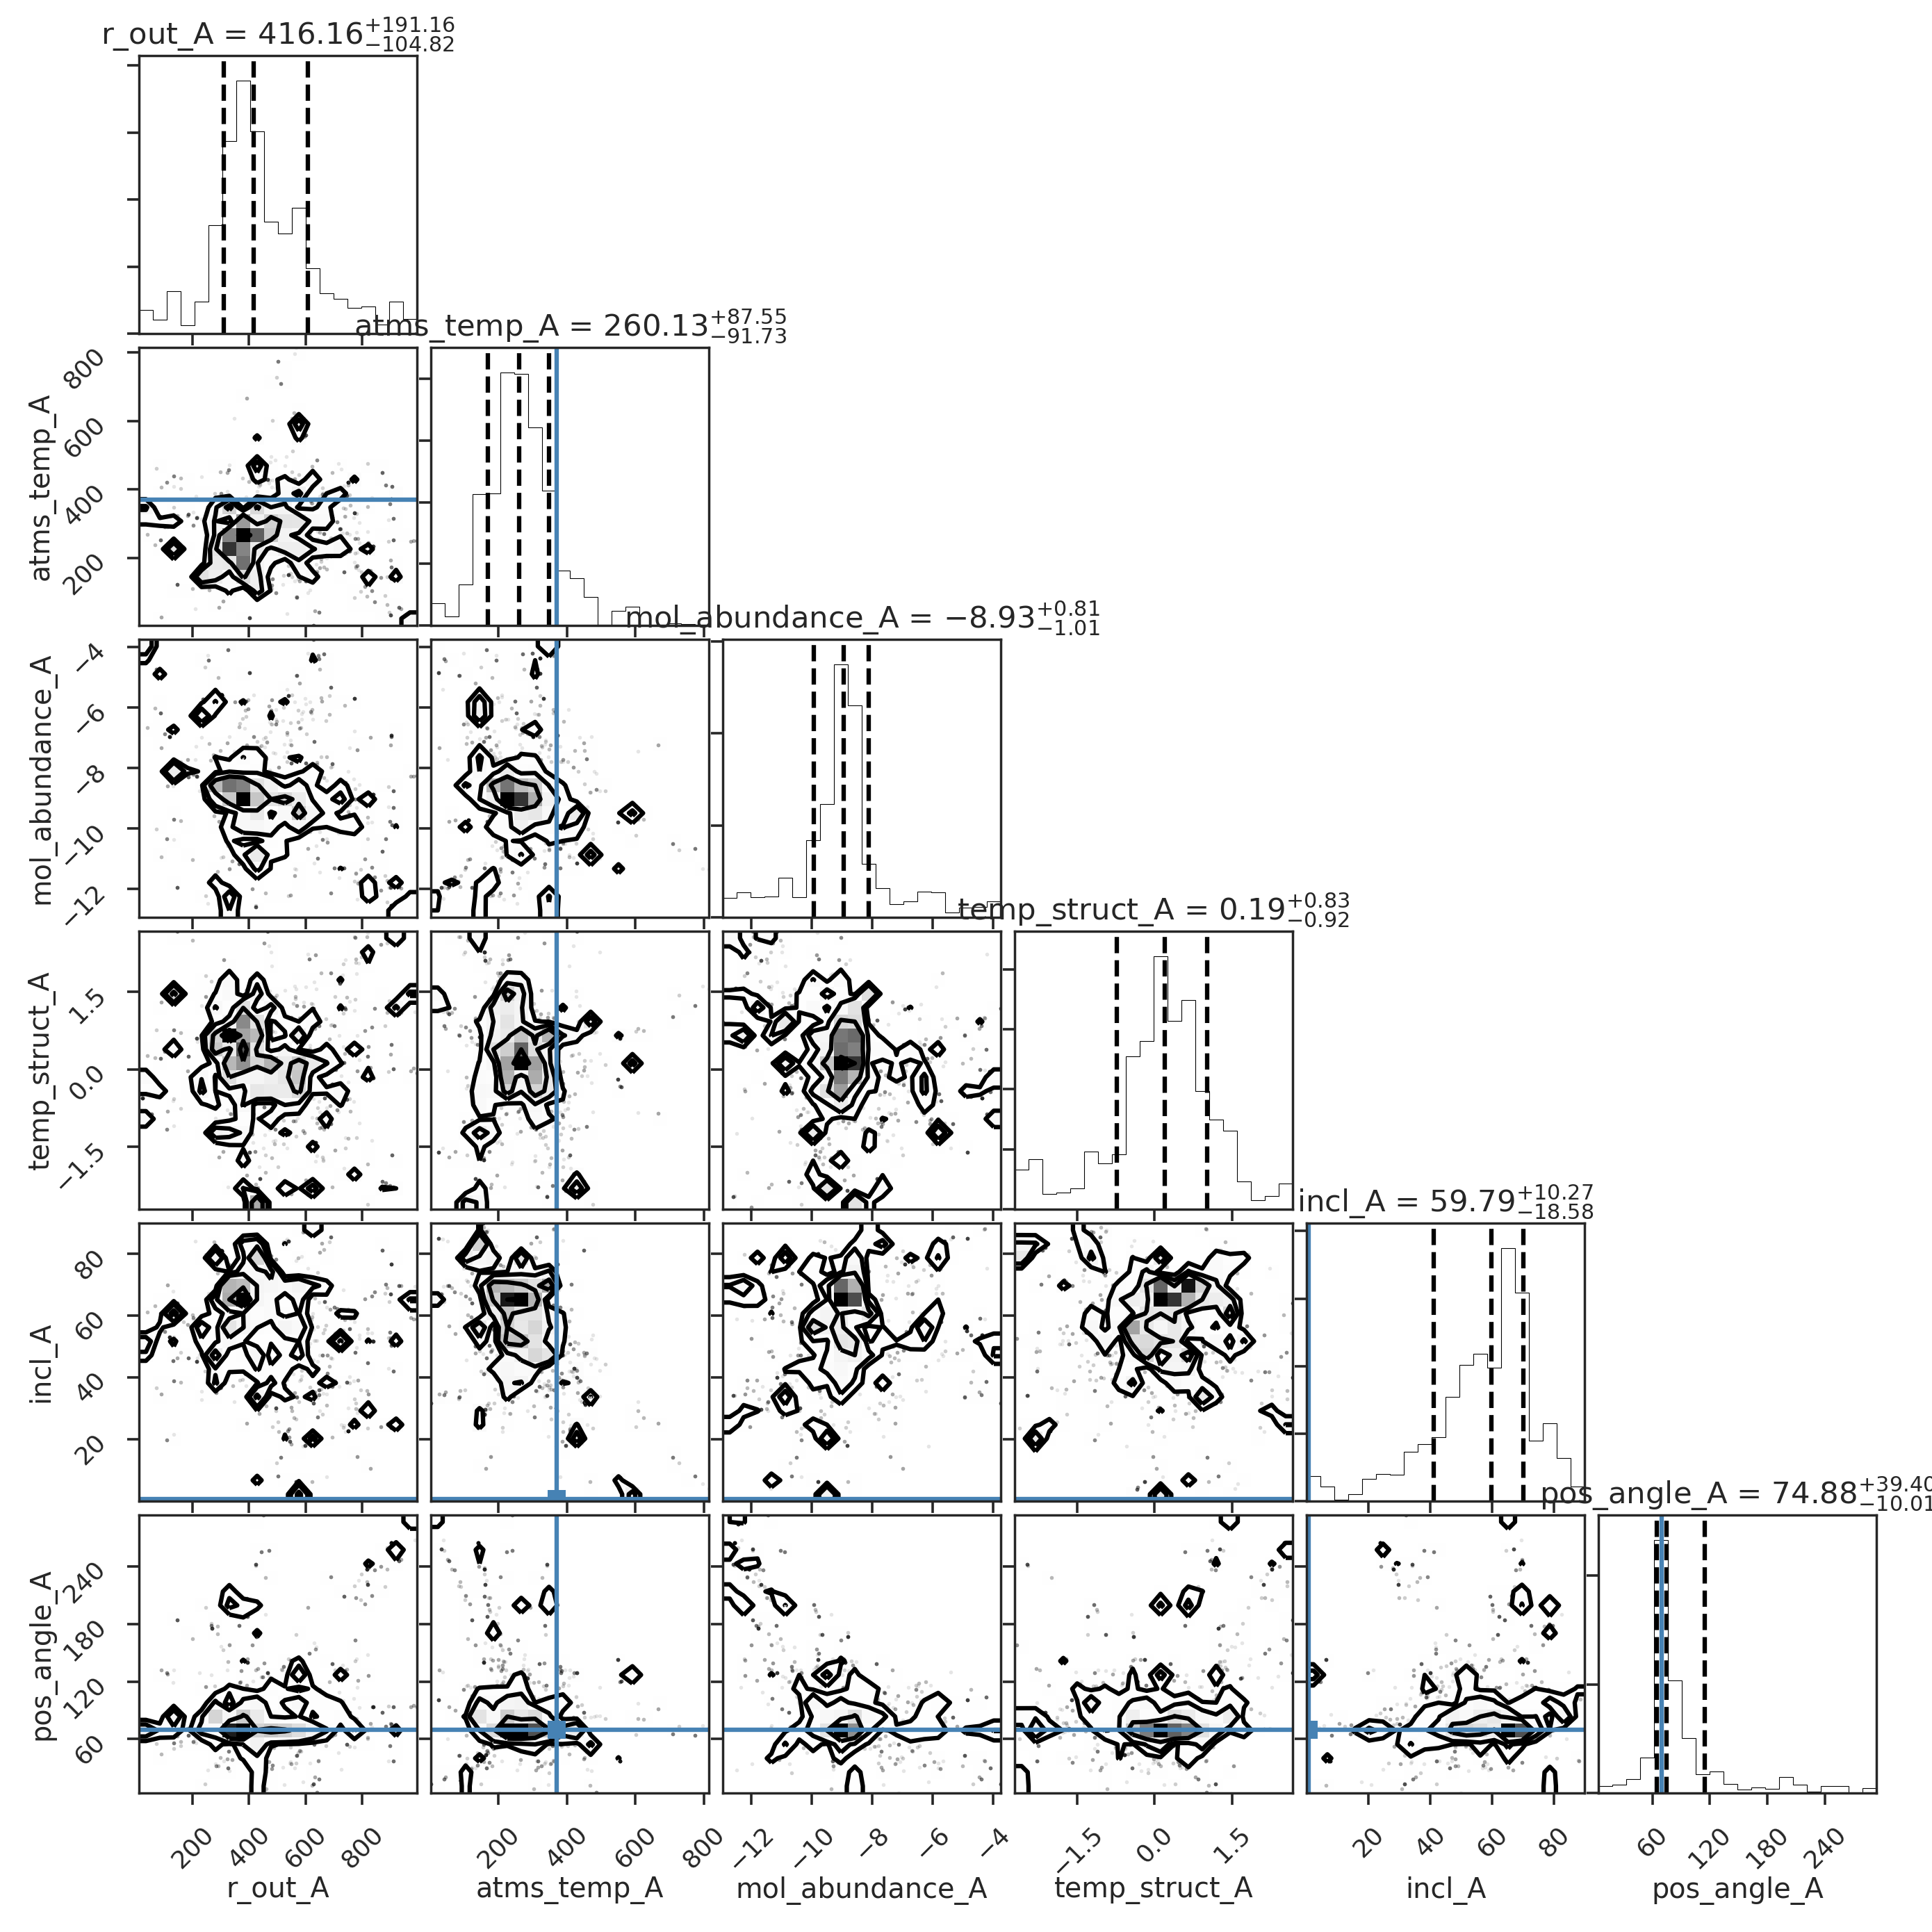
\includegraphics[width=0.49\linewidth]{cornerplot-diskA.png}}\hfill%
%   \subcaptionbox{Disk B fits \label{fig:corner_b}}{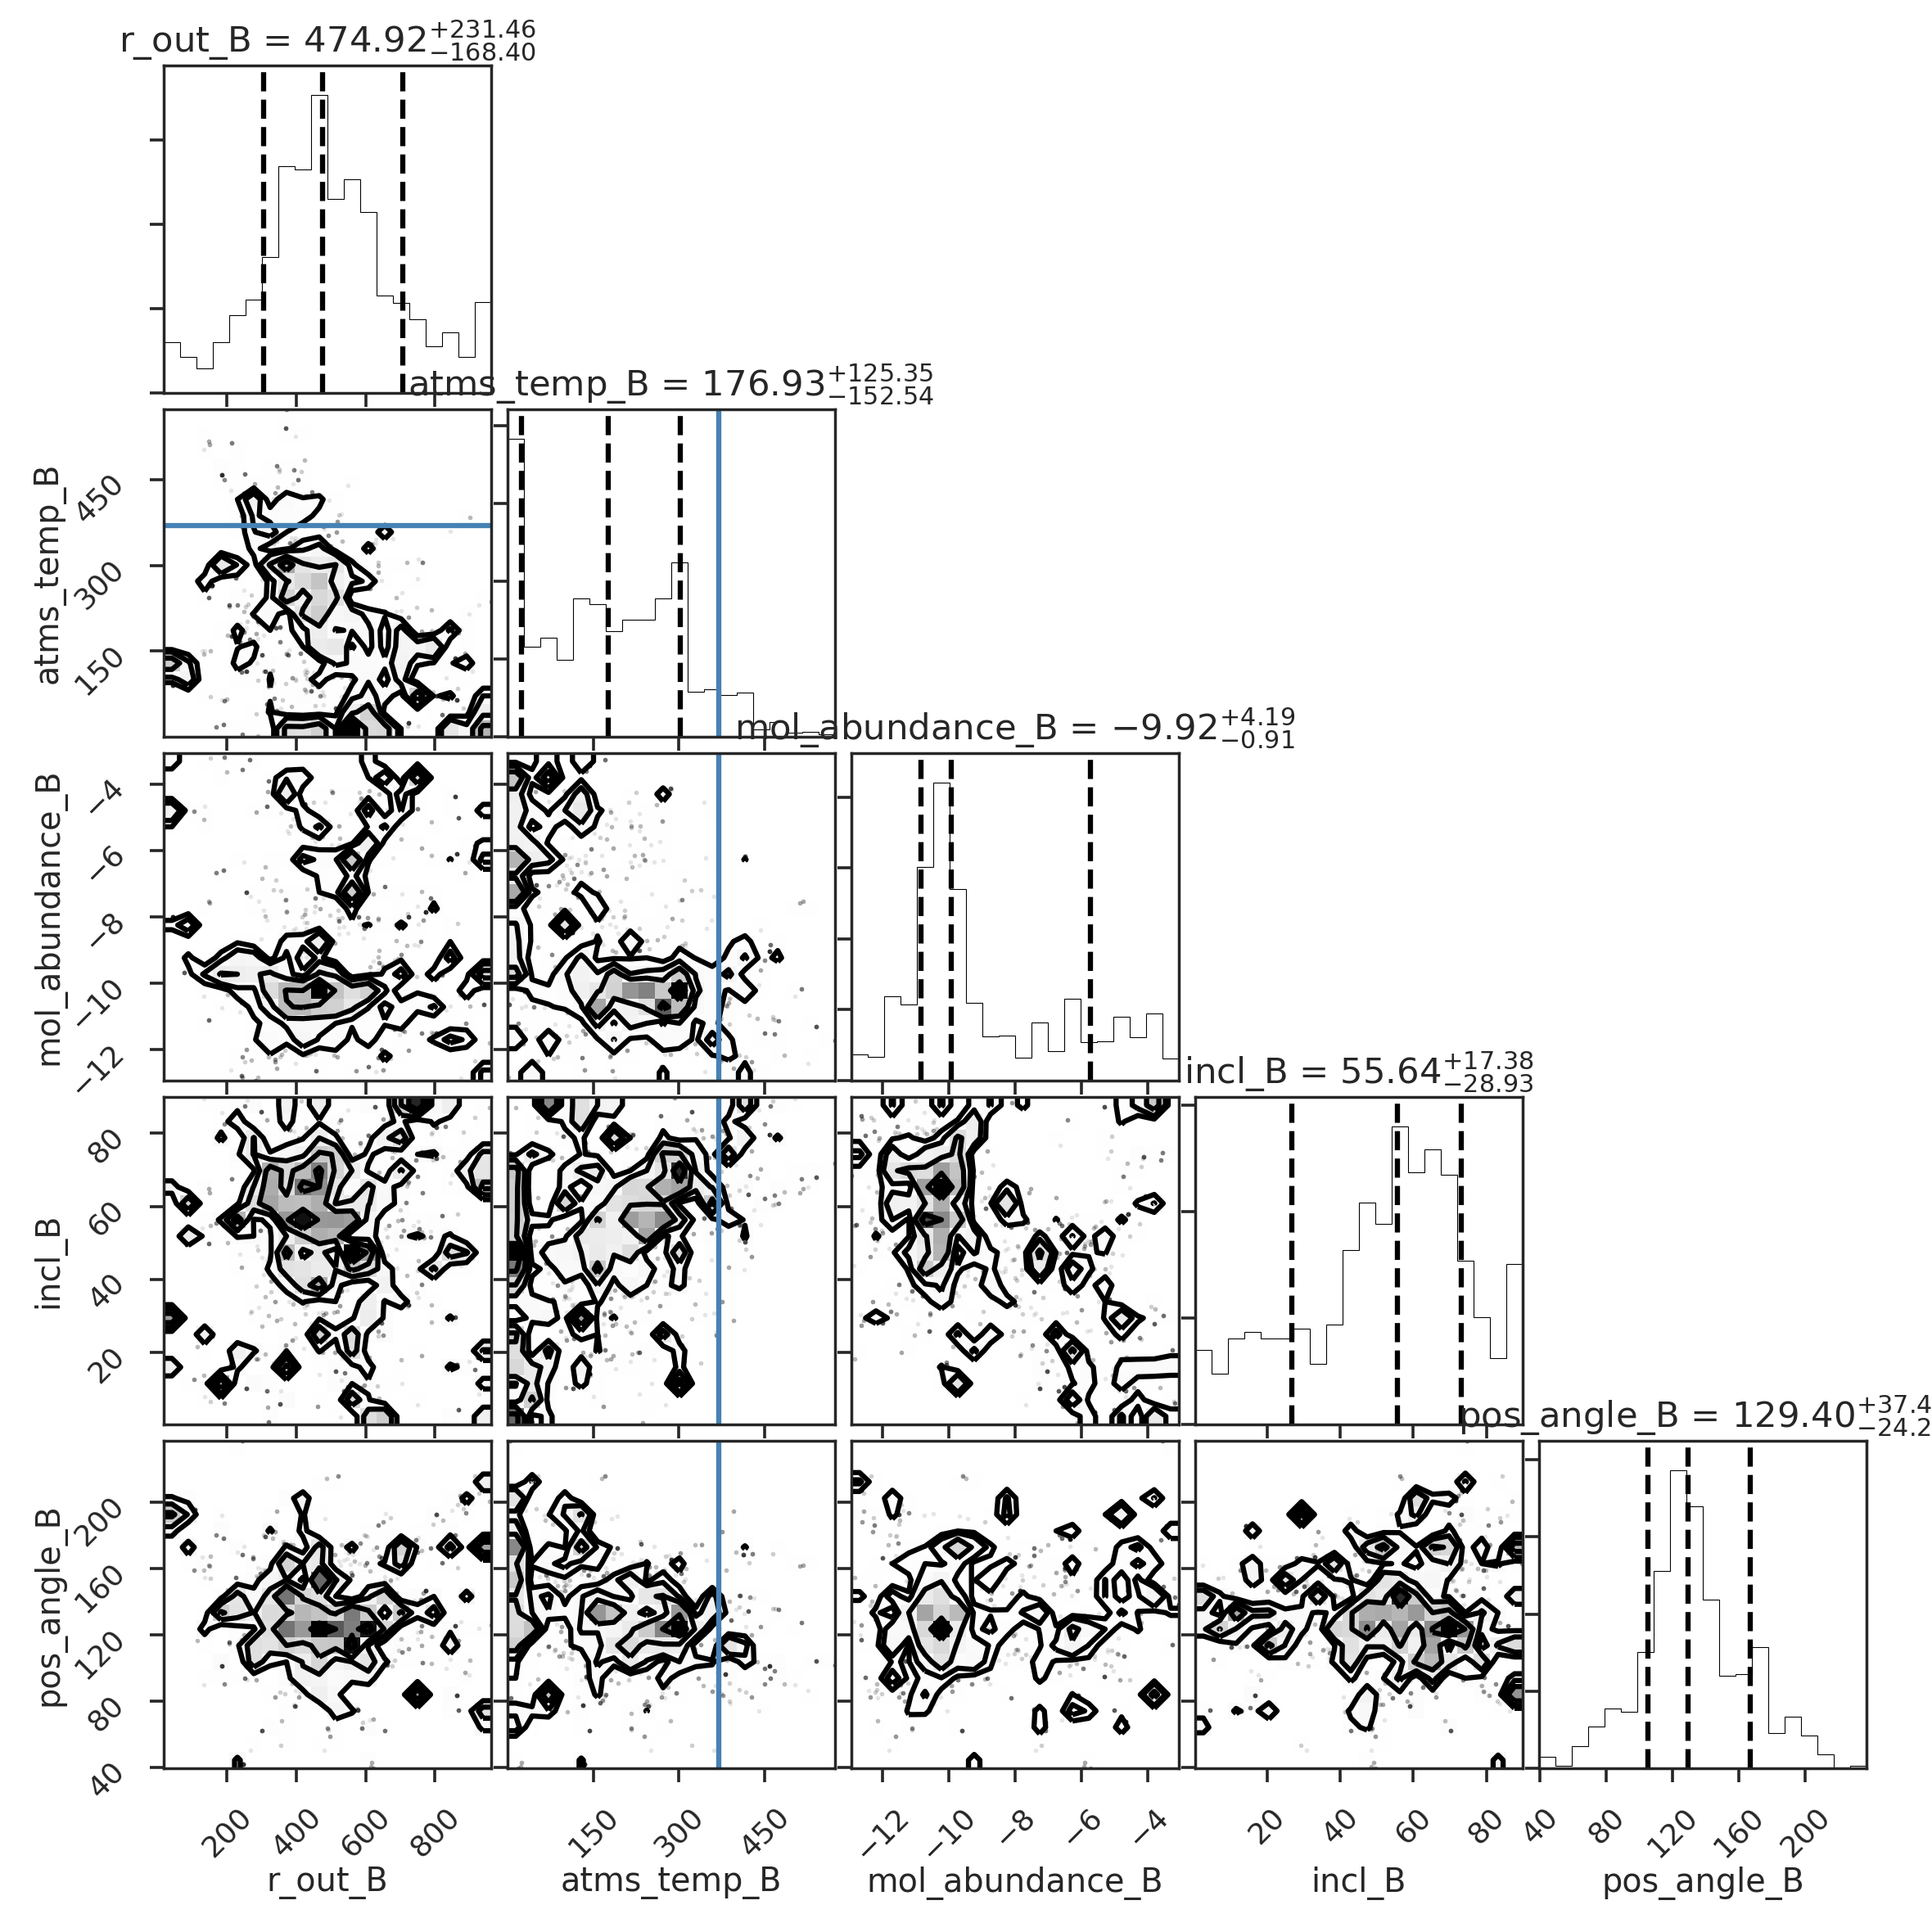
\includegraphics[width=0.49\linewidth]{cornerplot-diskB.png}}%
%   \hspace*{\fill}%
%   \caption{Since disk A and B's features are assumed to be independent, we may generate corner plots for each of their parameter spaces individually. Some analysis REWORK when new plots are added.}
%   \label{fig:co_corner_plots}
% \end{figure}




%% ~~~ DISK STRUCTURES PLOTS ~~~~~~~~~~~~~~~~~~~~~~~~~~~~~~~~~~~~~~~~~~~~~~~~~~~


\begin{figure}[htp]
  \centering
    \hspace*{\fill}%
    \subcaptionbox{CO}{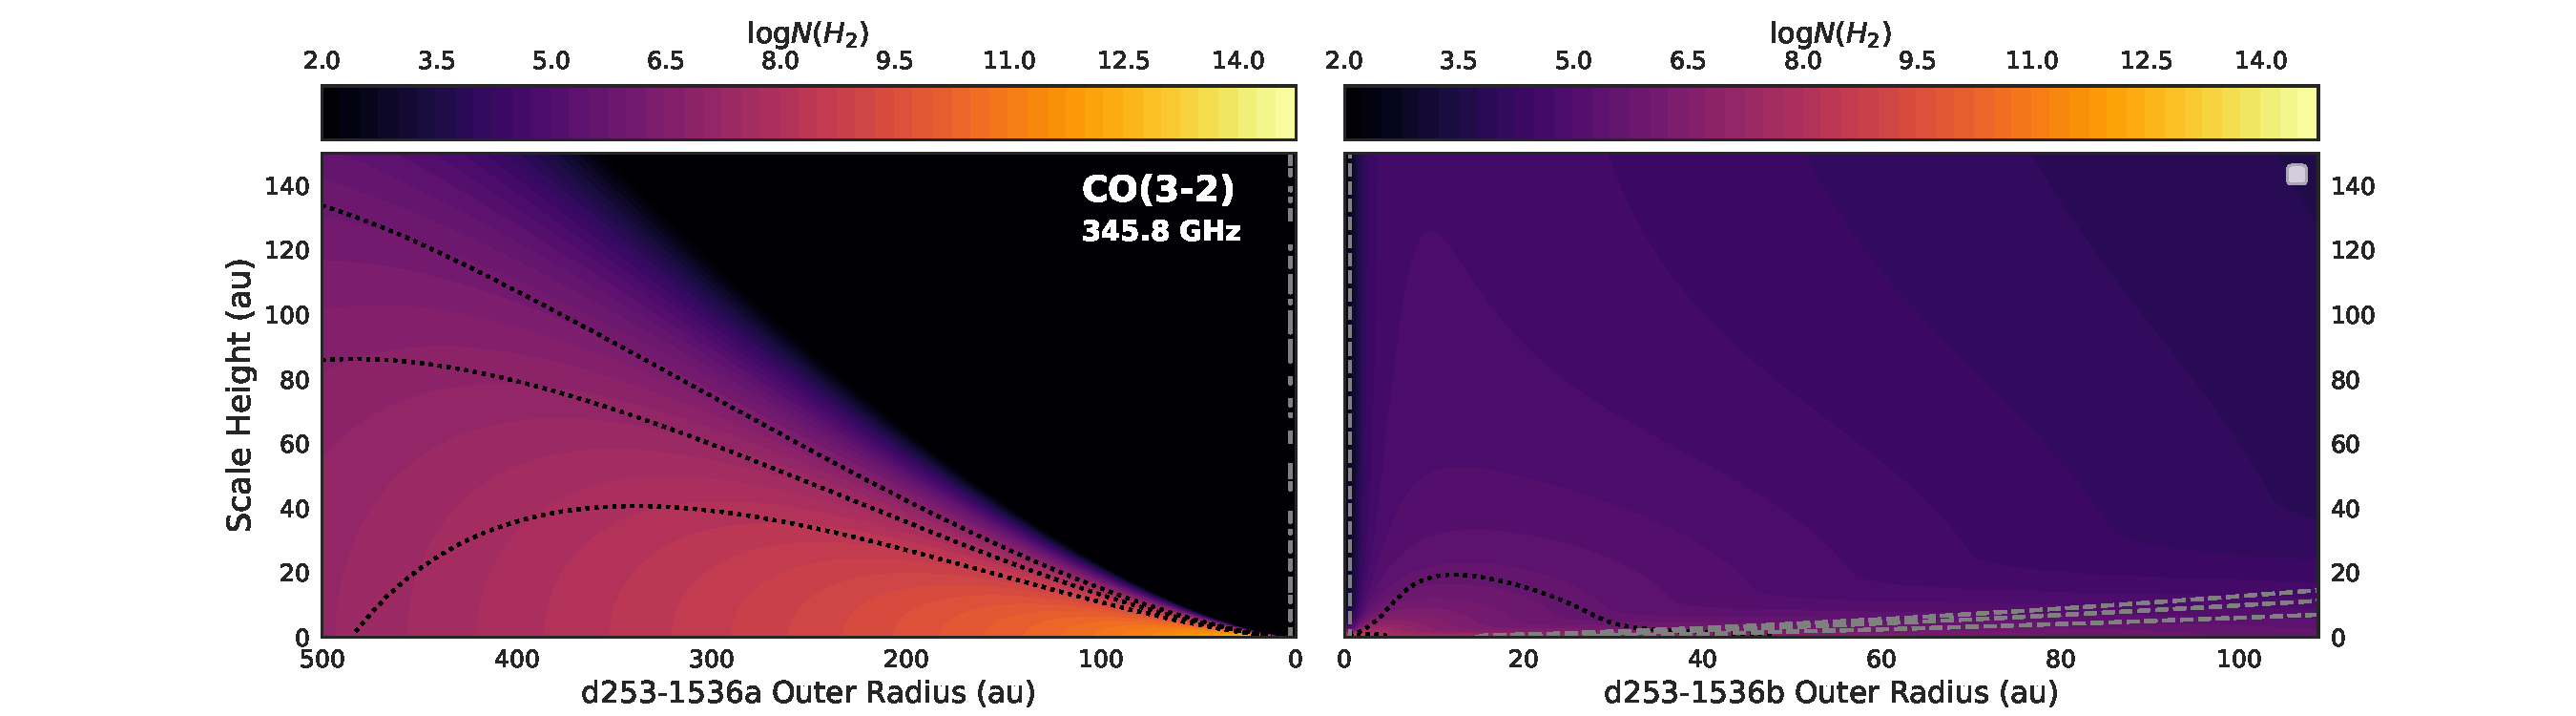
\includegraphics[width=\linewidth]{diskstructures-co.pdf}}\vfill%
    \subcaptionbox{\hco}{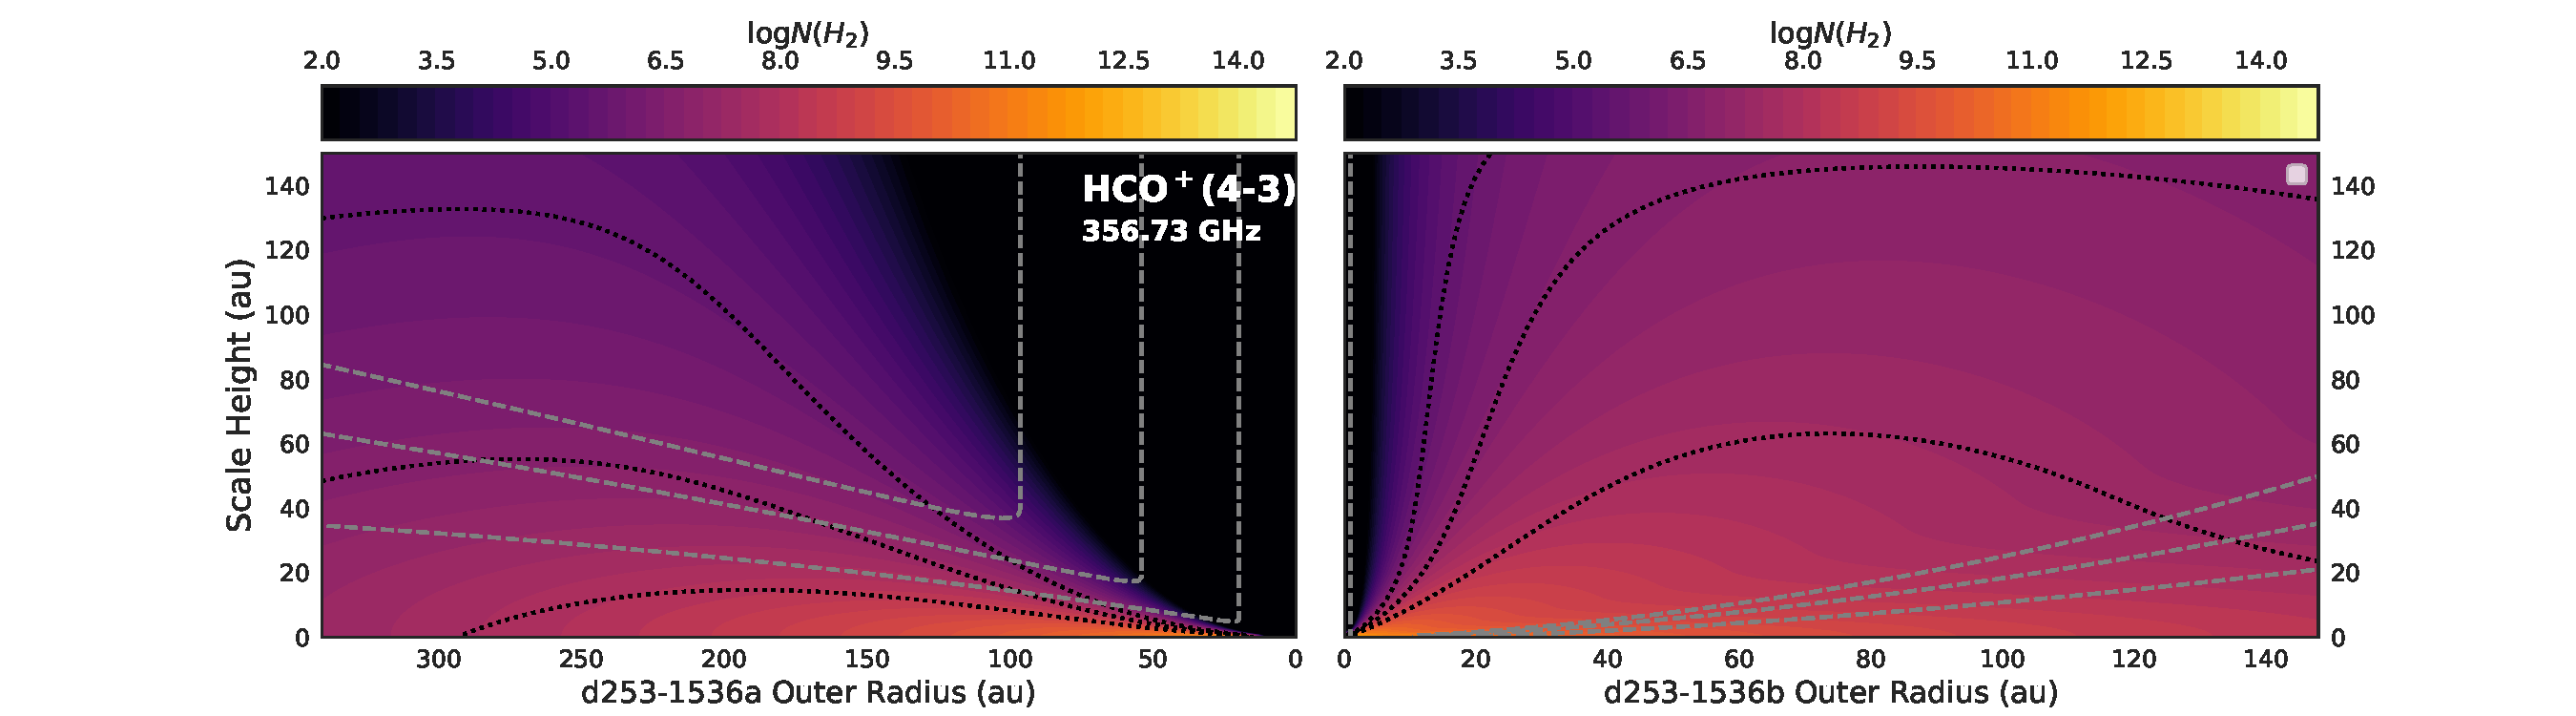
\includegraphics[width=\linewidth]{diskstructures-hco.pdf}}\vfill%
    \subcaptionbox{HCN}{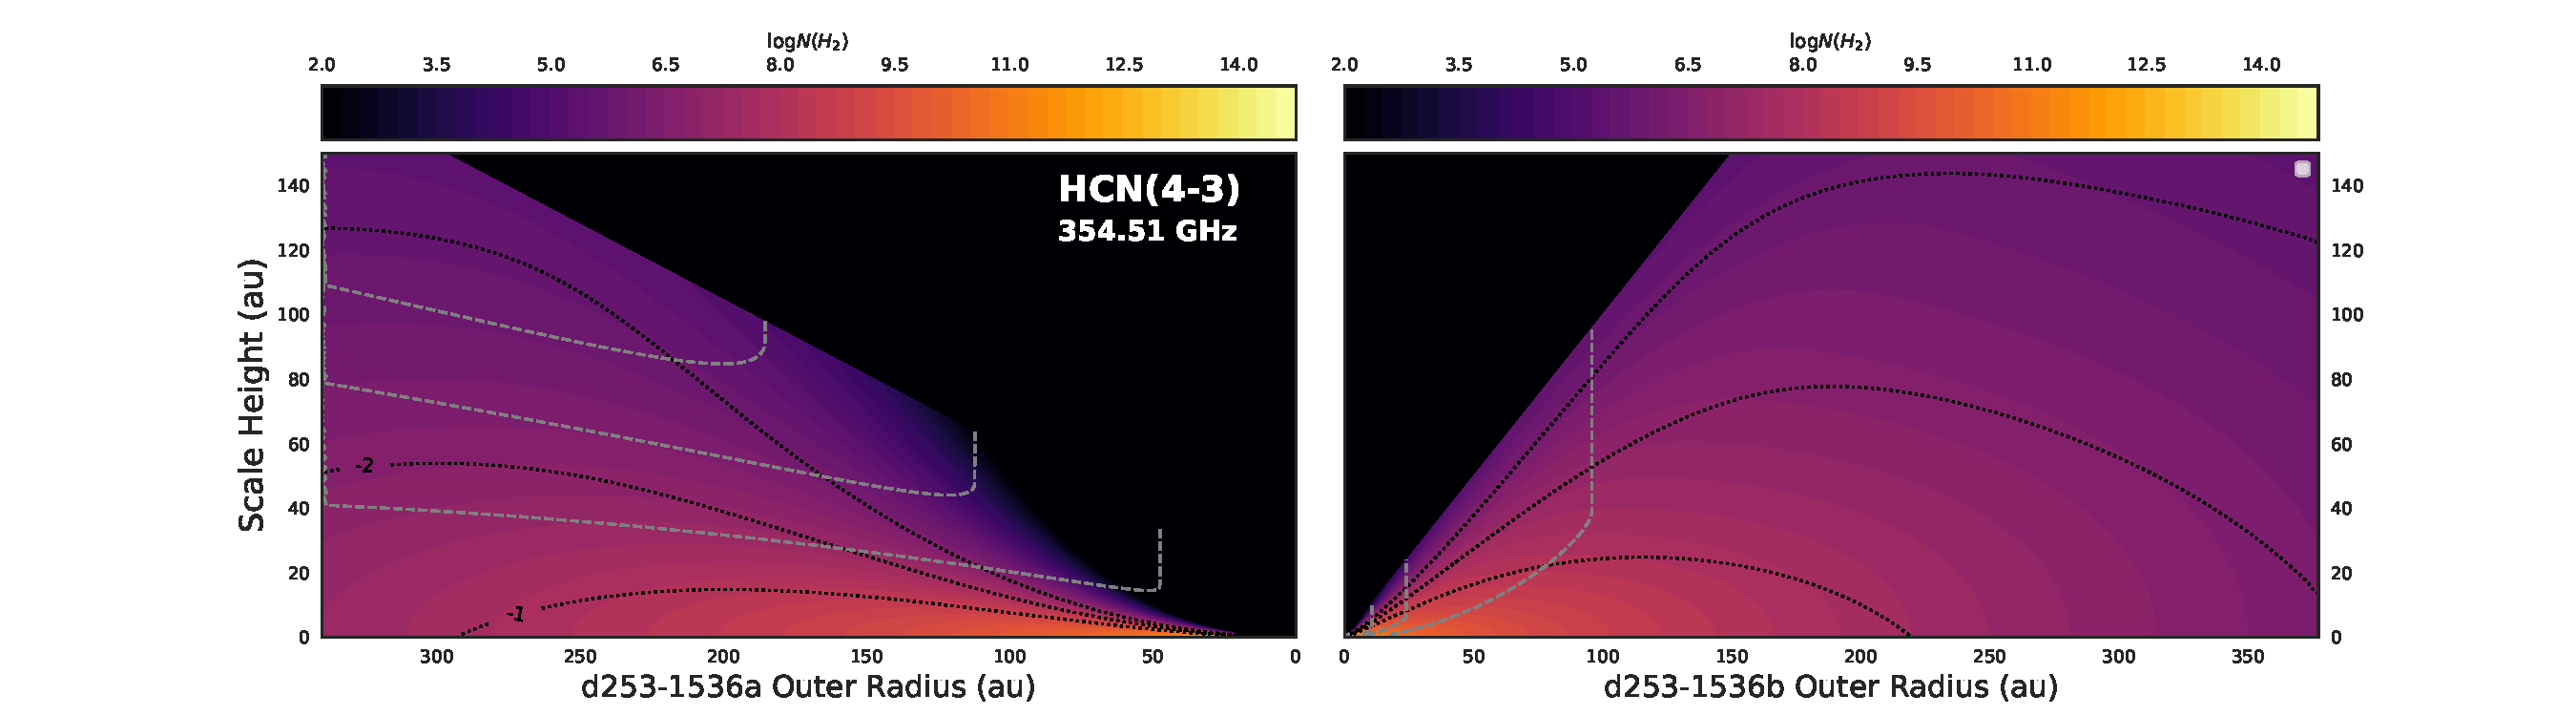
\includegraphics[width=\linewidth]{diskstructures-hcn.pdf}}%
    \hspace*{\fill}%
    \caption{Density and temperature profiles for the best-fit models for CO, \hco, and HCN.}
    \label{fig:bf_disk_strs}
\end{figure}

% \begin{itemize}
%   \item \textsc{RA/Dec Offsets} ($\Delta \delta, \Delta \alpha$): The positional offsets from image center for each disk, in arc-seconds. Originally fit with a Gaussian centroid, these offsets were validated/refined with a narrow-range grid search.
%   \item \textsc{Systemic Velocity} (v$_{\text{sys}}$): The radial velocity of each disk, in km s$^{-1}$. Initialized at values drawn from \cite{Williams2014}, these were also validated/refined using a narrow-range grid search.
%   \item \textsc{Distance} ($d$): The distance to the sources, in parsecs. Drawn from Gaia DR2 catalogue.
%   \item \textsc{Inner Radius} ($r_\text{in}$): Each disk's inner radius. Since these disks show no evidence of their interiors being carved out, we do not fit for an interior ring and allow the disks to extend almost all the way in to their stars.
%   \item \textsc{Turbulence Velocity} ($v_{\text{turb}}$): The speed of the turbulence in the disk. This value was left at its default, which \textit{maybe came from Flaherty}
%   \item \textsc{Vertical Temp. Str. Scale Height} ($Z_q$): The characteristic height, set at $r=150$ AU, determining the vertical temperature structure.
%   \item \textsc{Column Densities ([min, max])} ($[\sigma_1, \sigma_2]$): Min and max column density boundaries (corresponding to upper and lower boundaries) of molecular zone, in units of 1.59$\times10^{21}$ particles cm$^{-2}$
%   \item \textsc{Freeze-out Temperature} (T$_\text{FO}$): \textit{Wait why is this never used in my code.}
%   \item \textsc{Stellar Mass} (M$_\star$):
%   % \item \textsc{x} (y):
% \end{itemize}



% The End
